\chapter{Regresores y Clasificadores}
\label{ch:ClasificadorRedes}

\section{Introducción}

El concepto de \textit{Inteligencia Artificial} (\textit{IA}) en los últimos años ha tomado un nivel elevado de relavancia debido a la inclusión en nuestras vidas de tecnologías que presumen de ciertas 
capacidades o características especiales. Específicamente se anuncian como tecnologías inteligentes, capaces de brindarnos apoyo en la resolución de problemas cotidianos simples y también situaciones más complejas, las 
cuales se podrían considerar posibles de resolver exclusivamente para un humano. Sin embargo, actualmente en las computadores y teléfonos inteligentes encontramos asistentes virtuales que parecieran tener un comportamiento 
lógico y racional, en las calles encontramos vehículos capaces de llevar a su dueño a su destino sin que él tenga que poner sus manos en el volante, entre muchos otros avances tecnológicos que han surgido en los últimos 
meses; y seguirán apareciendo todavía más y cada vez con mayores capacidades. Todos estos avances promocionados bajo la cualidad de funcionar mediente Inteligencia Artificial.

Para aspectos de ingeniería, la Inteligencia Artificial no es más que una rama de las Ciencias de la Computación. Desde mediados del siglo pasado, científicos del área de la computación se interesaron por la idea futurística 
y utópica de computadoras y máquinas inteligentes o independientes que pudieran realizar tareas de forma autónoma. Se desarrollaron una gran cantidad de modelos matemáticos teóricos acerca de cómo podría llegar a ser posible 
la existencia de tecnologías de ese tipo. Sin embargo, la ingeniería en general aún era inmadura como para tener la capacidad de implementar un sistema de dichas características.

Desde las primeras propuestas teóricas en las décadas de 1940 y 1950 de los cientifícos McCulloch y Pits sobre las primeras redes neuronales artificiales, que no podían pasar de ser simplemente modelos teóricos debido a la 
inexistencia de \textit{hardware} capaz de realizar ese tipo de operaciones matemáticas, hasta las actuales tarjetas \textit{GPU} (\textit{Graphics Processing Unit, Unidad de Procesamiento de Gráficos}) utilizadas en 
\textit{computación acelerada}, capaces de realizar procesamiento en paralelo y ejecutar complejas redes neuronales procesando simultáneamente millones de parámetros \cite{gpuHP} \cite{gpuNVIDIA}. Todo este proceso ha sido gradual y ha requerido del 
avance conjunto tanto de los modelos matemáticos como del hardware. Y ahora tenemos a nuestra disposición y convertidas en realidad esas ideas primitivas sobre computadoras y máquinas inteligentes.

La investigadora Elaine Rich define la IA como la rama de las Ciencias de la Computación que se encarga del estudio de cómo lograr que las computadoras sean capaces de realizar tareas que de momento un humano las puede ejecutar 
mejor \cite{ElaineRichIA}. Esta definición implica un panorama absolutamente general pero que difícilmente perdera validez con el paso de los años debido a que define de una manera muy simple pero muy certera lo que es y lo 
que se busca con el desarrollo de la IA.

De forma más específica, más allá de una definición general de IA, lo importante es conocer que aplicaciones prácticas se pueden generar con la IA, y consecuentemente qué problemas nos puede ayudar a resolver, ya sean problemas 
que aún no han sido resueltos por los humanos o que ya se pueden resolver pero la IA representa una solución más eficiente \cite{ertel}. Algunas de las aplicaciones más reconocidas de la IA se enlistan a continuación.

\begin{itemize}
    \item \textit{Computer Vision}. Se refiere al procesamiento digital de imágenes usando técnicas de IA. Los usos más comunes para este tipo de procesamiento son enfocados al reconocimiento de patrones en una imagen dada, 
    es decir, poder determinar el tipo de objetos existentes en una imagen o incluso el reconocimiento facial para la identificación de personas. 
    \item \textit{Natural Language Processing}. Refiere a Procesamiento de Lenguaje Natural. Esta área va enfocada a entrenar y automatizar sistemas computacionales para que adquieran la capacidad de reconocer y entender las 
    diversas formas de comunicación que usamos los humanos.
    \item \textit{Sistemas de Clasificación}. Son modelos matemáticos optimizados con el propósito de realizar reconocimiento de patrones dado un conjunto de datos conocidos de un conjunto de variables, con el fin de poder 
    identificar el tipo de entorno, persona u objeto que se está analizando.
    \item \textit{Neural Networks}. Refiere a Redes Neuronales. Son modelos matematicos no lineales los cuales debido a su naturaleza intrínseca de no linealidad, permiten ser útiles en un número diverso de aplicaciones.
    Permiten realizar procesamiento digital de imágenes o audio, algoritmos de clasificación, sistemas de control automático, optimización y automatización de procesos, sistemas de detección de errores, algoritmos predictivos 
    para control de procesos, modelos de regresión, entre muchas otras.   
\end{itemize}

Para la realización de este trabajo de tesis se he hecho uso principalmente de Redes Neuronales con arquitecturas específicas para que puedan funcionar como clasificador. La elección de estos modelos en específico se debe 
a la mayor complejidad de las ecuaciones matemáticas que se pueden obtener con una red neuronal, lo cual es cierto que en lo referente a cálculo computacional resulta una tarea que requiere un número mayor de operaciones, 
sin embargo, al tener ecuaciones matemáticas con mayor número de términos es posible generar patrones de clasificación mejor optimizados o ajustados a los datos reales del proceso de potabilización analizado.

En este capítulo se exponen los fundamentos matemáticos de los modelos de clasificación basados en inteligencia artificial, iniciando con las ecuaciones fundamentales para un algoritmo de regresión lineal. Después, 
se exponen las ecuaciones para el método de optimización de descenso por gradiente, el cual supone una parte importante para la implementación del modelo final de clasificación de calidad del agua que se busca desarrolllar.
Posteriormente, se explica la teoría referente a redes neuronales, pasando por la explicación sobre los parámetros importantes en la definición de su arquitectura, así como sus funciones de activación y cómo se relacionan 
con los temas previamente explicados. Finalmente, se exponen las ecuaciones matemáticas para el proceso de entrenamiento de una red neuronal, en el cual se busca ajustar el valor de los pesos sinápticos de la red mediante 
técnicas iterativas de minimización de la magnitud del error en el modelo. 

\section{Modelo de Regresión Lineal}

En Matemáticas, una \textit{regresión} tiene como objetivo estimar el valor de 1 o más variables \textit{target} continuas \textit{t}, dado un vector N-Dimensional \textit{x} de variables de entrada \cite{bishop}.

El concepto de la regresión lineal es tener un conjunto de datos de entrada y explicar o predecir las salidas como una combinación lineal de las variables o datos de entrada. Es decir, lograr obtener una ecuación lineal 
optimizada que genere la mejor explicación o descripción posible de los datos de entrada. Se busca encontrar la relación entre las variables independientes y dependientes mediente el mejor ajuste posible de una línea recta 
con los puntos que representan los datos de entrada. Este lugar geométrico buscado se conoce como \textit{línea o plano de regresión} \cite{BigDataCandel}.

El modelo general de regresión lineal tiene la forma (\ref{eq:ecuacion701}).

\begin{equation}
	y(x,w)=w_0+w_1x_1+ \cdot \cdot \cdot +w_Dx_D
	\label{eq:ecuacion701}
\end{equation}

Es decir, \textit{y} es la variable target que se busca predecir mediante una combinación lineal de un número \textit{D} de variables de entrada. 

La \autoref{fig:figura700_1} muestra un ejemplo básico en 2 dimensiones.

\begin{figure}[h]
	\centering
	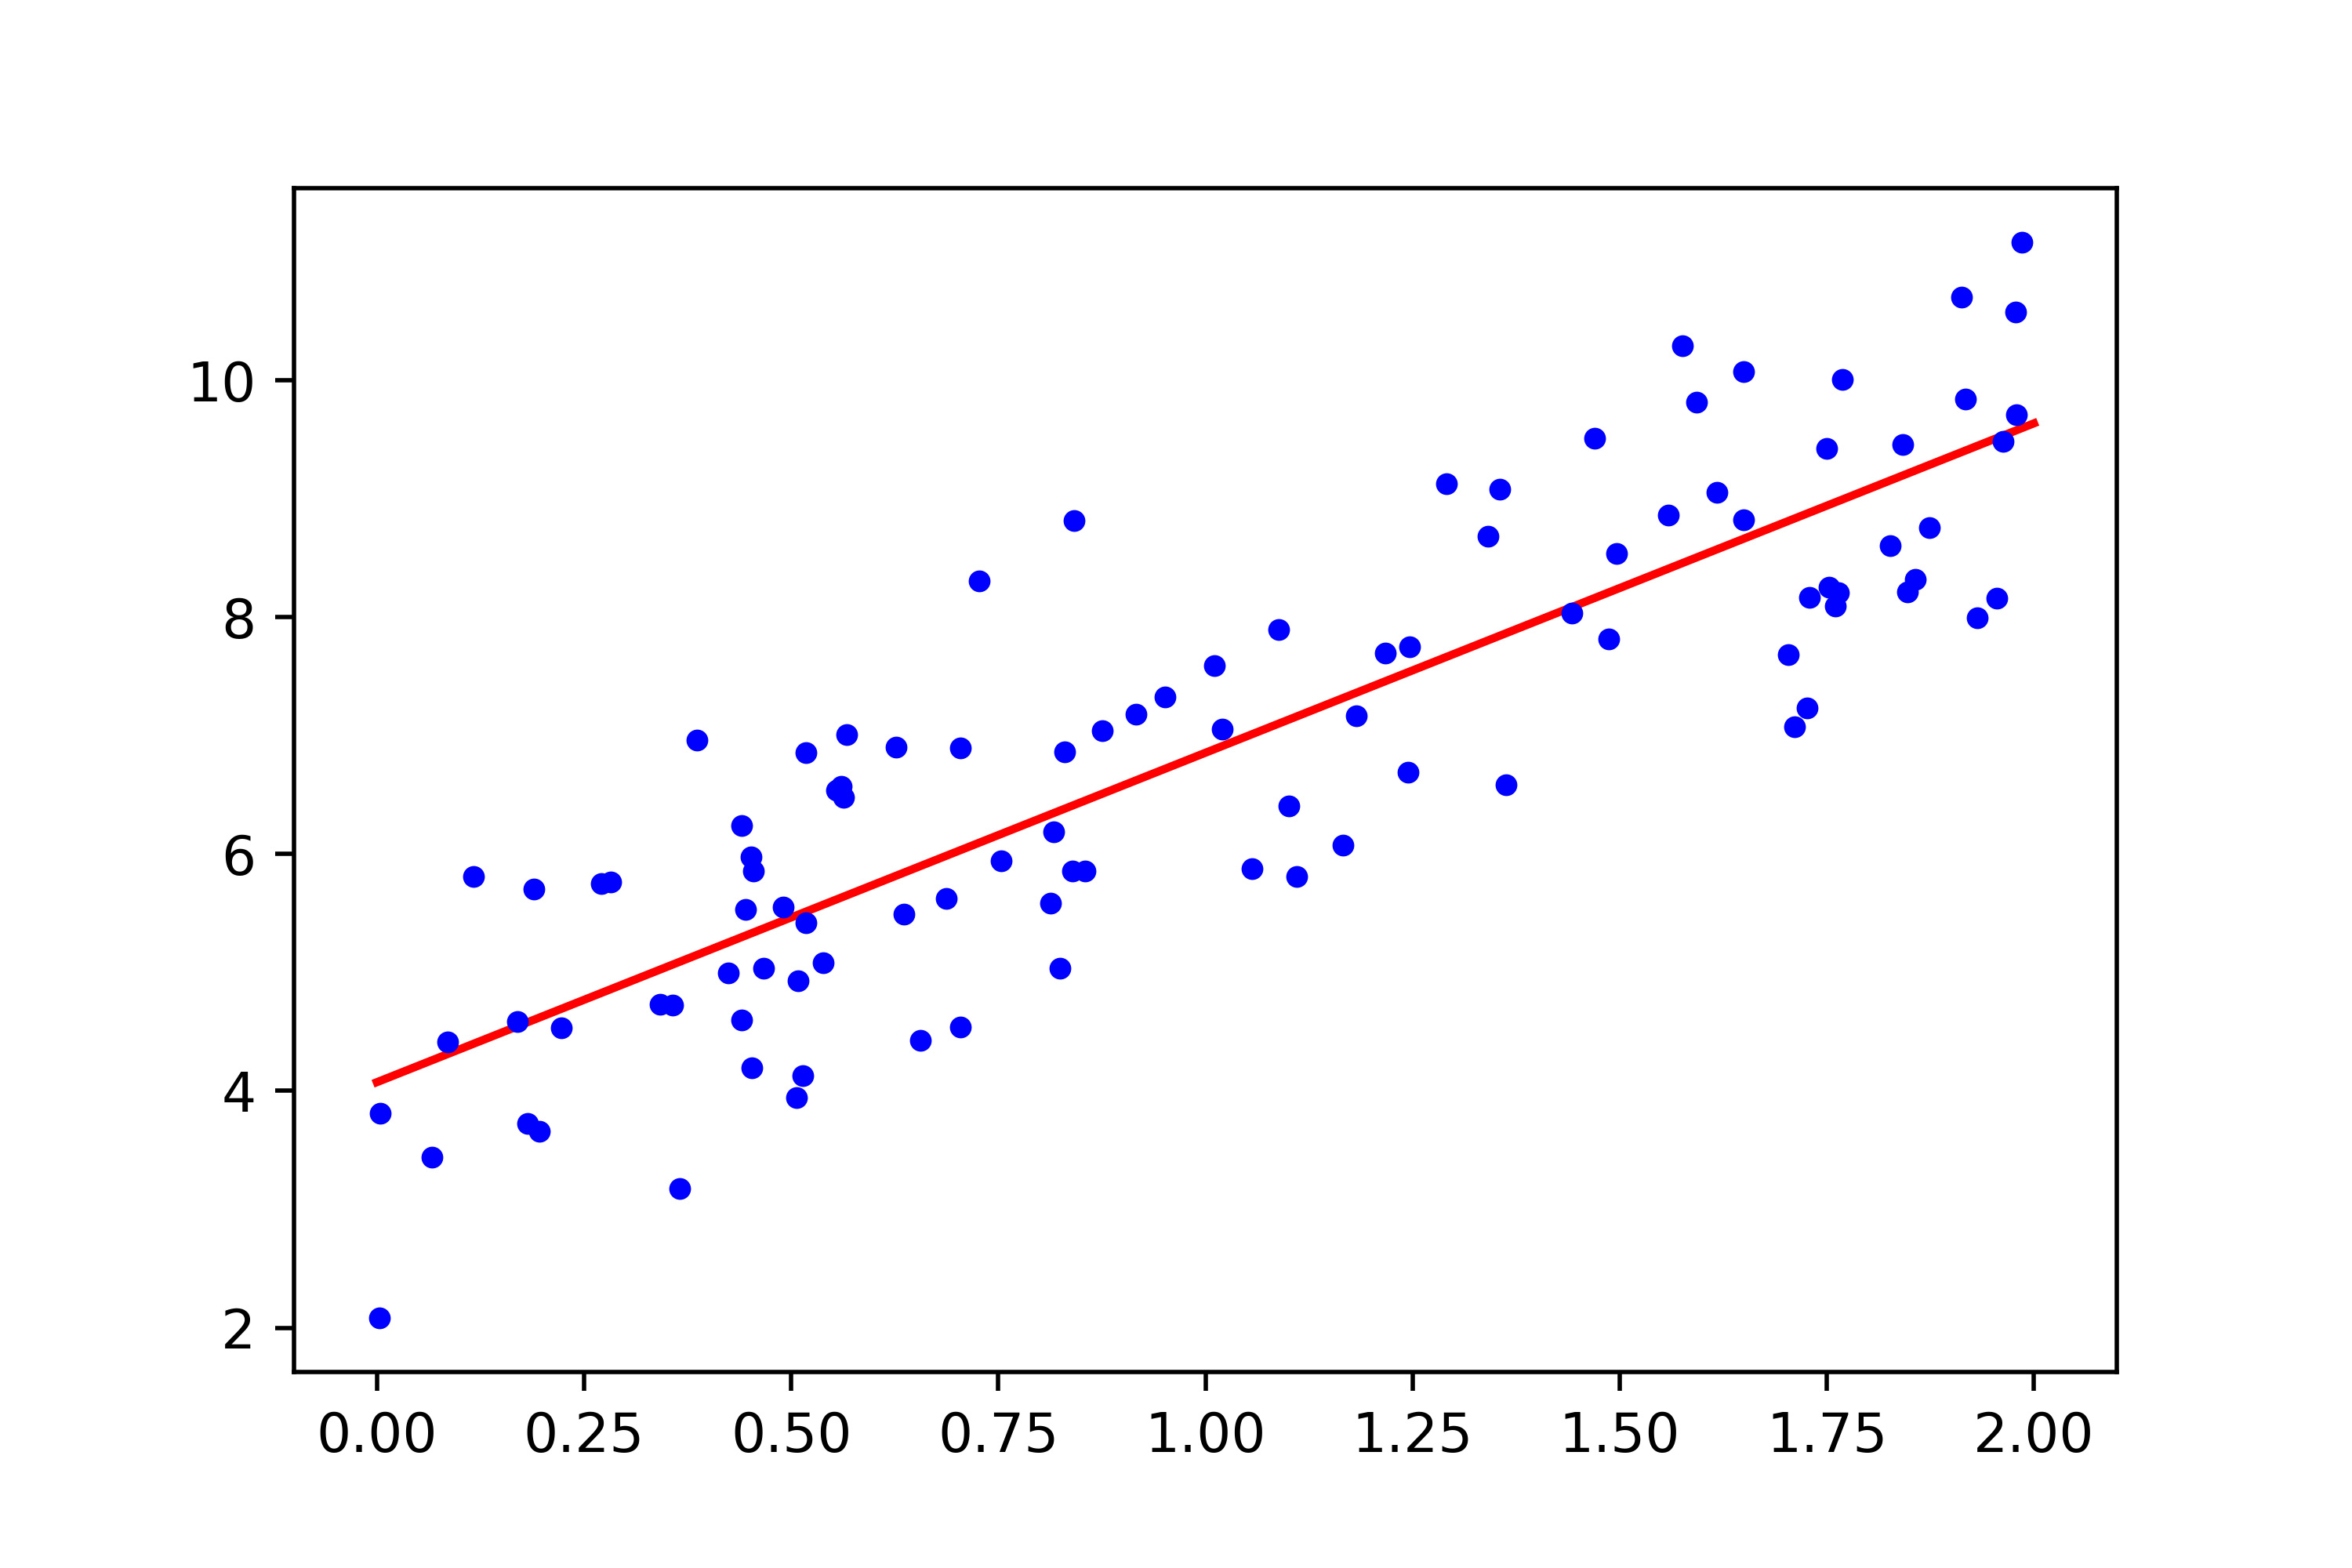
\includegraphics[scale=0.7]{imgss144.png}
	\caption{Aproximación de un conjunto de datos usando una línea de regresión}
	\label{fig:figura700_1}
\end{figure}

En la \autoref{fig:figura700_1} se tiene un diagrama de dispersión con los puntos o datos de 2 variables cualesquiera. Supongamos que se busca una función matemática que pueda tener este mismo comportamiento generado por 
estos datos. Si se quisiera tener una ecuación que igualara de forma perfecta esta tendencia y el lugar geométrico trazado cruzara por todos los puntos, probablemente habría que recurrir a un ejercicio de interpolación 
polinómica, pero esto implicaria generar un polinomio complejo de grado superior.  

Si no es necesario replicar de manera perfecta el comportamiento mostrado por los puntos graficados, y resulta suficiente con generar una expresión matemática que siga la misma tendencia sin necesidad de cruzar por cada 
uno de los puntos de la gráfica, entonces se puede recurrir a un ejercicio de regresión lineal que pueda generar una función matemática cuyo lugar geométrico generado sea una recta en 2 dimensiones, tal y como se muestra 
en la \autoref{fig:figura700_1}. Para este ejemplo mostrado, se observa que la recta de color rojo trazada no cruza por casi ninguno de los puntos, sin embargo, logra replicar la tendencia del comportamiento de una forma 
general.

El objetivo de este método es hallar los valores óptimos del vector de pesos \textbf{w}, dado de la forma (\ref{eq:ecuacion702}).

\begin{equation}
	\textbf{w}=(w_0,w_1,...,w_D)
	\label{eq:ecuacion702}
\end{equation}

\subsection{Método de Mínimos Cuadrados para la Regresión Lineal}

Una vez que se tiene la forma descriptiva de los datos de las variables para las cuales se busca una aproximación mediante regresión lineal, lo que sigue es encontrar una ecuación lineal que permita representar la mayor 
cantidad de puntos dados por los datos de entrada. Se busca que dicha ecuación lineal pase lo más cerca posible por cada uno de los puntos, para lo cual es necesario optimizar los valores de los coeficientes o pesos de la 
combinación lineal. El método de \textit{Mínimos Cuadrados} permite dar un paso a una posible solución para dicha optimización de los coeficientes de la combinación.

La idea del método de mínimos cuadrados consiste en calcular la diferencia entre las predicciones hechas por el modelo de regresión y los valores reales de la variable \textit{target}. Dado que el valor del \textit{error} 
arrojado por estas diferencias puede generar números negativos, dichas diferencias deben ser elevadas al cuadrado para posteriormente realizar la sumatoria de todos estos valores de error, y finalmente el valor de dicha 
suma dividirlo entre el valor total de muestras del conjunto de datos. A este último resultado se le conoce como \textit{error cuadrático medio} (\textit{MSE, Mean Square Error}), y entre menor sea su valor, mejor será el 
ajuste realizado para los pesos del modelo \cite{PinedaPertuzML}.

El error cuadrático medio (MSE) se define de la forma (\ref{eq:ecuacion703}).

\begin{equation}
	MSE=\frac{1}{m} \sum_{i=1}^{m}e_s
	\label{eq:ecuacion703}
\end{equation}

donde $e_s$ se define de la forma (\ref{eq:ecuacion704}).

\begin{equation}
	e_s=(y_{pred} - t)^2
	\label{eq:ecuacion704}
\end{equation}

Es decir, el cuadrado de la diferencia de el valor predicho y el valor target deseado.

\subsection{Descenso por Gradiente}

El método de \textit{descenso por gradiente} es un algoritmo iterativo usado en regresión lineal para encontrar el valor óptimo de los pesos de la combinación lineal que minimicen una \textit{función de costo}. Para cada 
iteración que se ejecuta este algoritmo, se realiza una actualización en el valor de los pesos \cite{PinedaPertuzML}. Para ilustrar cómo es que opera este método se usa como apoyo la \autoref{fig:figura700_2}.

\begin{figure}[h]
	\centering
	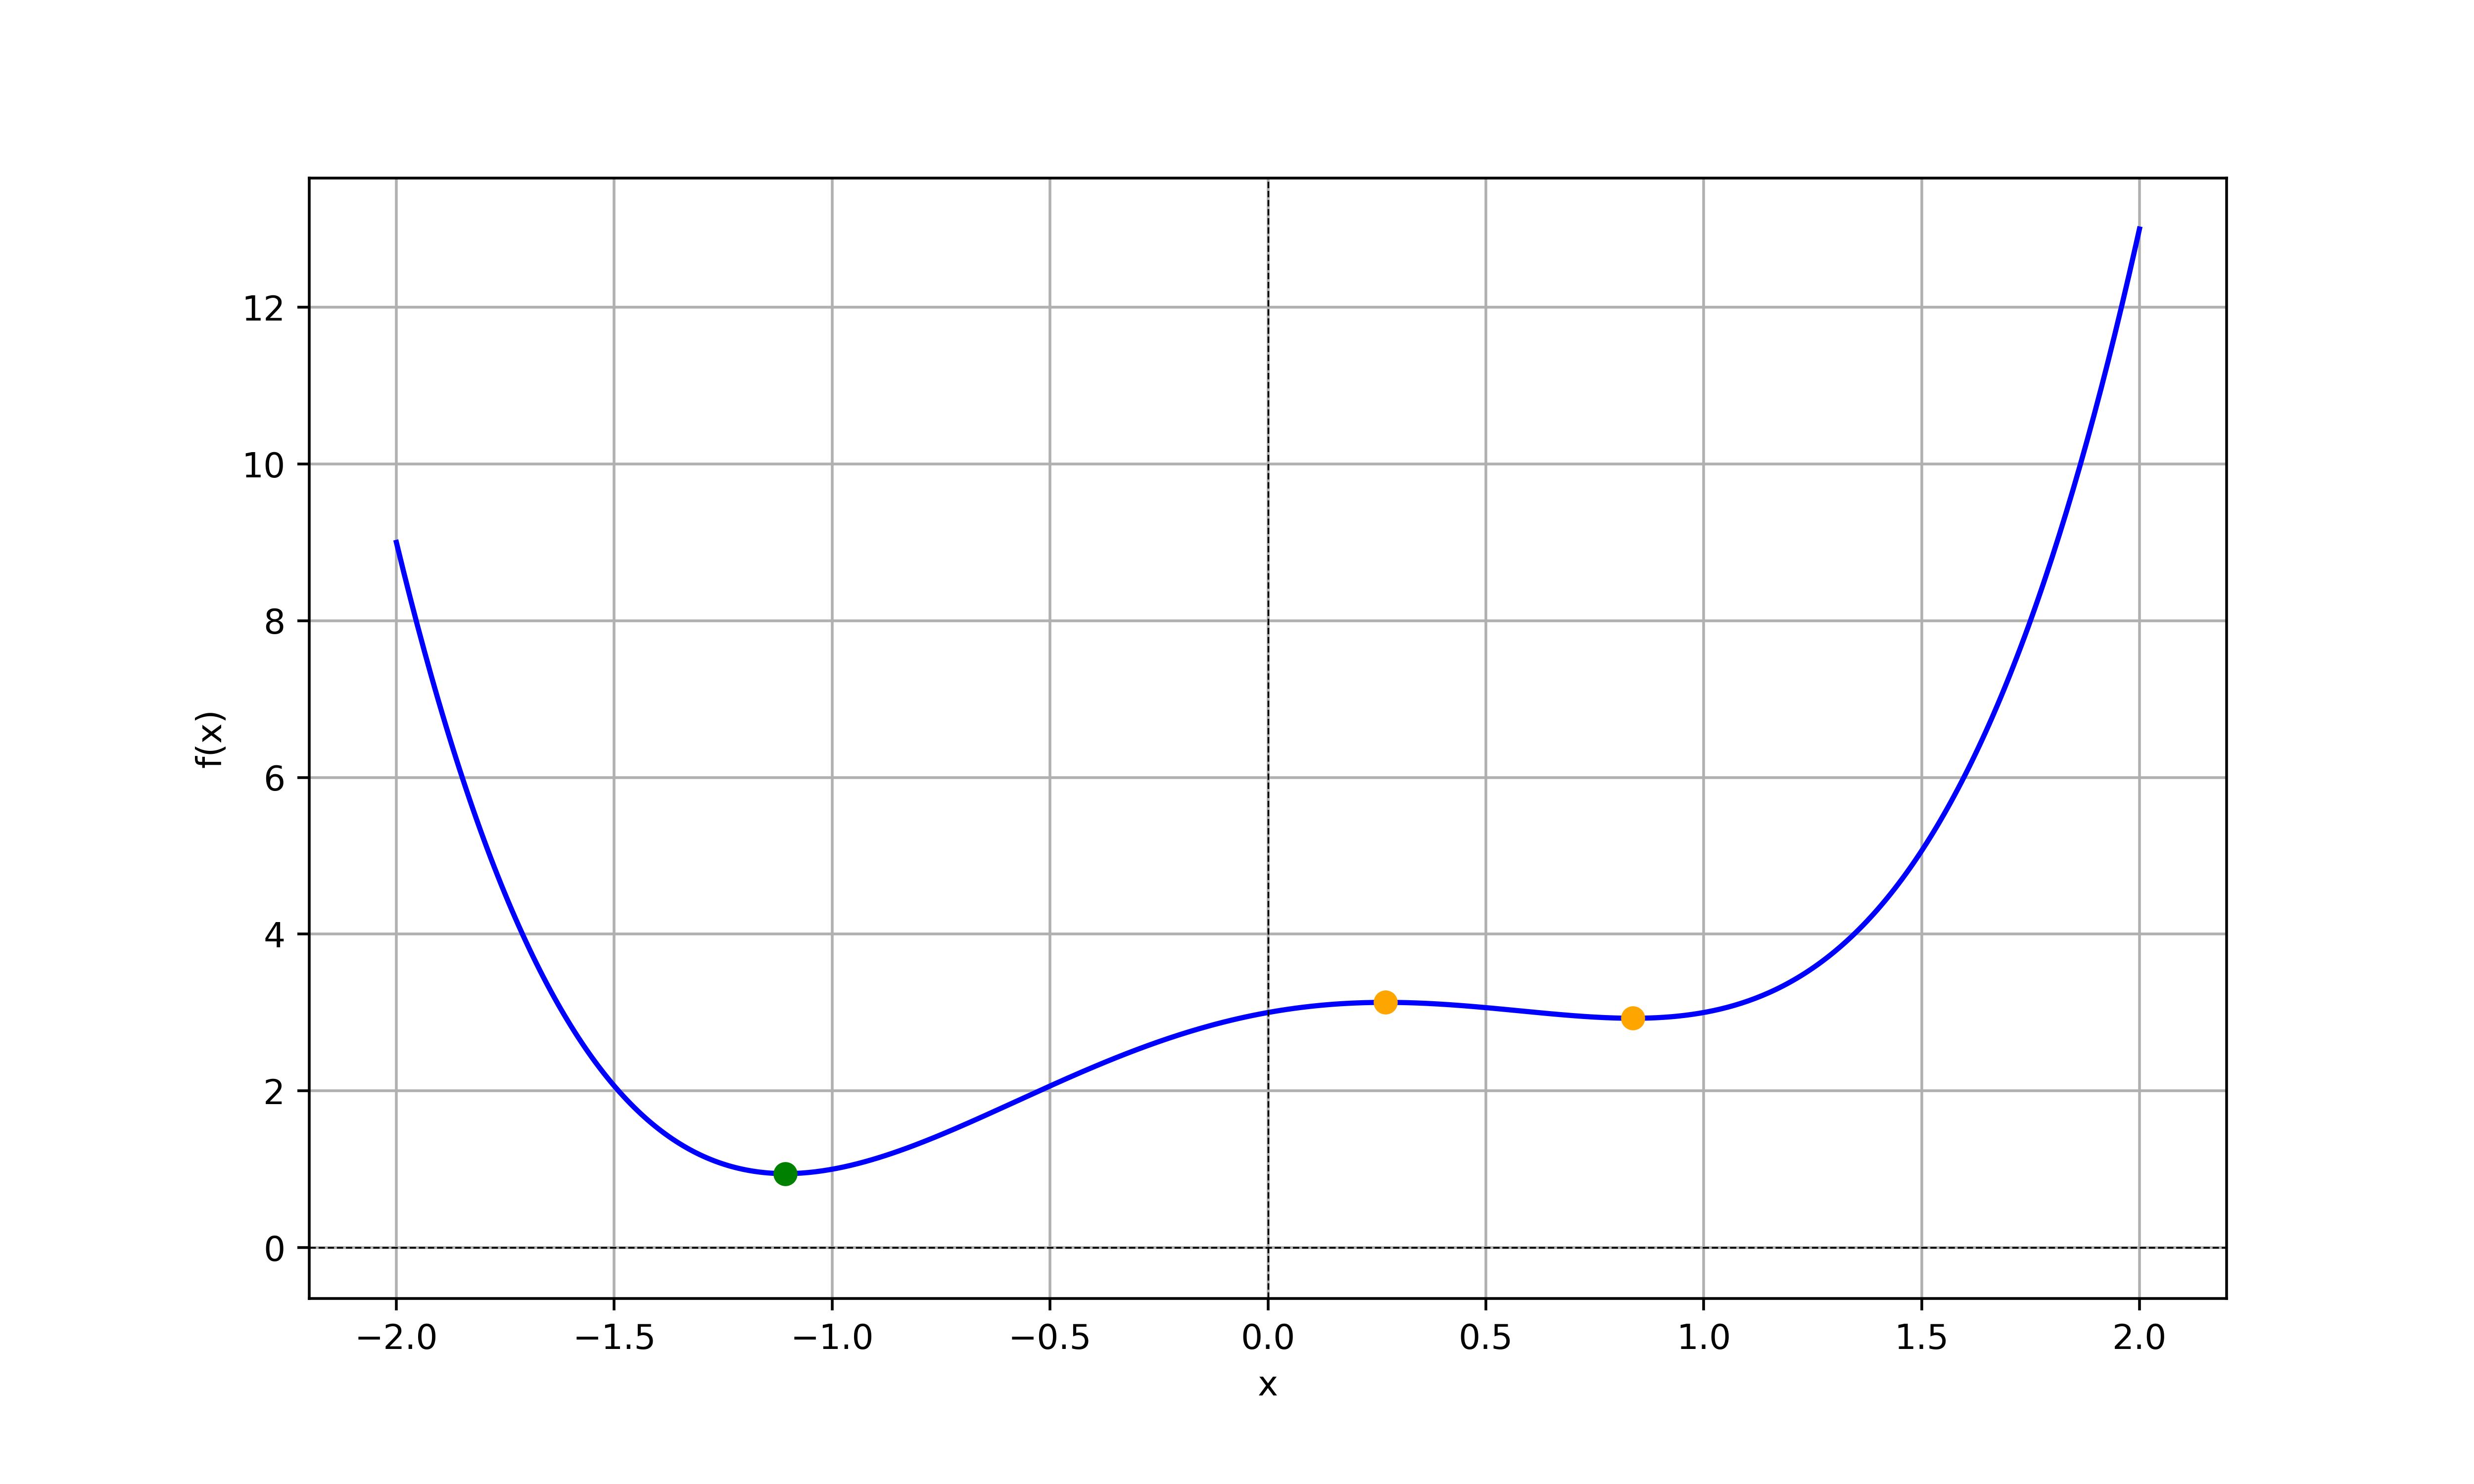
\includegraphics[scale=0.6]{imgss206.png}
	\caption{Ejemplo de una función de costo}
	\label{fig:figura700_2}
\end{figure}

De forma simple, una función de costo es una expresión matemática que nos indica el MSE, y para esta función lo que se busca es encontrar su \textit{mínimo global}. Es decir, el valor más pequeño que puede tomar la variable 
dependiente de la función. Tomando como ejemplo la \autoref{fig:figura700_2}, donde se grafica una hipotética función de costo, la idea de este método es encontrar el valor de \textit{x}  que genere el valor 
más pequeño de la función \textit{f(x)}. Con esto, teniendo que \textit{x} representa un peso y \textit{f(x)} representa el MSE, lo que se está logrando es encontrar el valor del peso que genera la máxima 
minimización del error para la regresión lineal.

Por lo tanto, una función de costo se define de la forma (\ref{eq:ecuacion705}).

\begin{equation}
	J(\textbf{w})=\frac{1}{m} \sum_{i=1}^{m}e_s
	\label{eq:ecuacion705}
\end{equation}

Donde $e_s$ tiene la forma (\ref{eq:ecuacion706}).

\begin{equation}
	e_s=(y_{pred} - t)^2
	\label{eq:ecuacion706}
\end{equation}

Es decir, las mismas ecuaciones que para el MSE.

Para este tema, es necesario realizar la definición de la herramienta matemática que nos ayuda a hacer posible este método de optimización.

El \textit{gradiente} de una función \textit{f} de \textit{n} variables se define de la forma (\ref{eq:ecuacion707}) \cite{CalculoVectorialLarson}.

\begin{equation}
	\nabla{f} (x_1,x_2,...,x_n)= \hat{x_1} \frac{\partial{f}}{\partial{x_1}} +\hat{x_2} \frac{\partial{f}}{\partial{x_2}} + ... + \hat{x_n} \frac{\partial{f}}{\partial{x_n}} 
	\label{eq:ecuacion707}
\end{equation}

Es decir, el gradiente de una función genera como resultado un campo vectorial, en donde cada uno de los términos es el producto de la derivada parcial de la función respecto a una de las variables independientes con su 
correspondiente vector unitario. 

La importancia de este resultado para la optimización de los pesos en la regresión lineal radica en la interpretación o efecto geométrico que pueden tener este campo vectorial evaluado en un punto cualquiera permitido para 
las variables independientes.

Un análisis a fondo de este campo vectorial del gradiente, arroja como resultado que dicho campo vectorial evaluado en un punto, ese vector resultante representa para ese punto la dirección y sentido del \textit{máximo incremento o ascenso} 
para la función \textit{f} \cite{CalculoVectorialDennisZill}. Es decir, el gradiente de la función evaluado en un punto nos indica la dirección a donde tendríamos que movernos si quisiéramos ascender de la manera más rápida
sobre la superficie n-dimensional dada por la función \textit{f}.

Podemos hacer una comparación de la función de costo \textit{J(w)} con la función \textit{f} a la cual se le aplica el gradiente. El gradiente nos permite encontrar la forma más rápida de ascender sobre la función que se 
está analizando, pero en la función de costo para la regresión lineal lo que se busca es llegar al punto más bajo, el ya mencionado mínimo global. Si el gradiente nos entrega la forma más rápida de ascender, entonces la 
forma más rápida para descender sobre la función de costo nos la entregaría el inverso aditivo del gradiente aplicado a la función de costo (\ref{eq:ecuacion708}).

\begin{equation}
	- \nabla{J(w)}= - \hat{w_1} \frac{\partial{J(w)}}{\partial{w_1}} - \hat{w_2} \frac{\partial{J(w)}}{\partial{w_2}} - ... - \hat{w_n} \frac{\partial{J(w)}}{\partial{w_n}} 
	\label{eq:ecuacion708}
\end{equation}

Es aquí con este resultado que encontramos cómo podemos generar el método de descenso por gradiente para la regresión lineal. En cada una de la iteraciones del algoritmo, se puede realizar una actualización de los pesos o 
coeficientes al dar pequeños \textit{pasos} en la dirección opuesta dada por el vector gradiente. El ejemplo clásico para este caso es imaginar el estar en la cima de una montaña y se desea descender hasta el punto más 
bajo de la misma, pero que el descenso sea de la forma más adecuada u óptima posible; cuando se está en las partes altas de la montaña, donde la pendiente es elevada, el descenso se puede hacer de forma más rápida al dar 
\textit{pasos más grandes}; caso contrario, cuando se está en puntos más bajos de la montaña donde la pendiente es menor, se tendrá que dar \textit{pasos más pequeños} \cite{PinedaPertuzML}.

Ahora supongamos que se tiene el vector de pesos de la forma (\ref{eq:ecuacion702}); iterativamente se desea encontrar sus valores que generen que la función de costo \textit{converga} hasta un valor mínimo o que se halla 
cumplido un valor umbral establecido previamente para el MSE. La ecuación (\ref{eq:ecuacion709}) expresa la modificación necesaria para el d-ésimo peso en cada iteración del algoritmo.

\begin{equation}
	w_D = w_D - \alpha \frac{\partial{J(w)}}{\partial{w_D}}
	\label{eq:ecuacion709}
\end{equation}

En la ecuación (\ref{eq:ecuacion709}) el factor $\alpha$ se denomina la \textit{tasa de aprendizaje} del algoritmo. Este factor representa el \textit{tamaño de los pasos} dados en el descenso para cada iteración.
Es decir, sirve para controlar cuánto se \textit{avanza} y se suele asignársele un valor en el rango de 0.0001 a 1, aunque a veces se suele asignar valores cercanos a 10 y el algoritmo funciona de mejor forma que para 
otros valores. La asignación de su valor se hace mediente prueba y error, considerando que un valor muy grande puede ocasionar que se produzcan \textit{saltos bruscos} de un lado a otro sobre la superficie de error \textit{J(w)},
provocando que el valor del error MSE se incremente y decremente continuamente y el algoritmo nunca alcance la convergencia. De la misma forma, un valor demasiado pequeño puede ocasinar que el algoritmo requiera un número 
muy elevado de iteraciones, lo cual en muchas ocasiones es un problema a nivel de cálculo computacional \cite{PinedaPertuzML}.

El proceso de iteraciones del algoritmo de descenso por gradiente se repite hasta que el valor del error MSE sea un valor muy pequeño cercano a 0; dado que es muy poco probable alcanzar el valor de 0 para el MSE, el 
algoritmo se suele controlar asignando un número límite de \textit{épocas} o iteraciones que logre generar un valor de MSE lo suficientemente bajo para los requisitos dados por la aplicación dada.

Para el caso de estudio de algoritmos de clasificación basados en redes neuronales, la optimización para minimización del error por descenso por gradiente será en nuestro caso el método empleado. Para el problema que se 
analiza en este proyecto, existen métodos de optimización más complejos, sin embargo el método de descenso por gradiente resulta suficiente y adecuado gracias a su eficiencia en casos donde se emplea una gran cantidad de 
datos para entrenamiento del modelo, lo que permite al mismo tiempo reducir la carga computacional. Adicionalmente, este método resulta adecuado en problemas donde no es necesario obtener una solución exacta, como en el 
caso de una red neuronal que se busca principalmente la mejor optimización posible.

\section{Modelos no Lineales para Clasificación}

En IA, un algoritmo de clasificación consiste en tomar un conjunto de características \textbf{x} de un objeto, proceso o ente, y dicho valor asignarlo a 1 de \textit{K} valores posibles \cite{bishop}. Es decir, por ejemplo, 
existen diferentes tipos de calzado dependiendo del uso que tendrá, consecuentemente cada clase diferente de calzado tendrá diferentes caracteristicas.

En los problemas de clasificación existen diversas maneras de usar los valores \textit{target} para poder representar las \textit{etiquetas} de clase, es decir, las diferentes clases o tipos que se manejan en un problema 
dado. Por ejemplo, en modelos probabilísticos, para el caso de únicamente 2 clases posibles, la forma más común es usar 1 sola variable target \textit{t} que tome 2 valores solamente, 0 y 1. De esta forma \textit{t=1} representa la clase \textit{$C_1$} y \textit{t=0} representará a la clase restante \textit{$C_2$}.
Un problema de este tipo se conoce como \textit{clasificación binaria} y un ejemplo simple sería la diferenciación en el sexo o genero de una persona, que puede tomar 2 clases posibles, hombre o mujer.

Para un valor de \textit{K} mayor a 2 clases posibles, \textit{clasificación multiclase}, es conveniente usar una variable \textit{t} que sea un vector de tamaño \textit{K}, de forma que si el clasificador arroja como resultado correcto la clase \textit{$C_j$}, 
entonces todos los elementos \textit{$t_k$} de \textbf{t} sean 0 y el elemento \textit{$t_j$} se le asigne un valor de 1 \cite{bishop}. Un ejemplo sería dado por (\ref{eq:ecuacion710}).

\begin{equation}
	\textbf{t}=(0,1,0,0,0)
	\label{eq:ecuacion710}
\end{equation}

%La ecuación (\ref{eq:ecuacion710}) podría representar un ejemplo de clasificación con 5 clases posibles, en el cual un vector de entrada específico entrega como resultado que la clase \textit{$C_2$} es la correcta para el 
%vector de entrada dado.

La ecuación (\ref{eq:ecuacion710}) podría representar un ejemplo de resultado de un algoritmo de clasificación con 5 clases posibles, en el cual el segundo elemento del vector correspondiente a la clase \textit{$C_2$} tiene 
un valor de 1 y los demás elementos del vector son 0, indicando que esa es la estimación del clasificador. Un ejemplo sería el caso de un modelo clasificador que analice imágenes de playeras y las clasifique de acuerdo a 
sus características; por ejemplo, playeras deportivas, playeras para eventos formales, playeras de tipo casual, playeras de pijama y playeras para entornos laborales. El clasificador analizaría las imágenes para determinar 
las características físicas y poder estimar el tipo de playera que se encuentra en la imagen.

Para tareas de clasificación, los modelos matemáticos usados en regresión lineal pueden ser de utilidad para generar nuevos algoritmos para generar los clasificadores. Para lograr esto, se puede establecer una generalización 
de los modelos para regresión al usar una función no lineal sobre la función lineal aplicada a los pesos o coeficientes del modelo (\ref{eq:ecuacion711}) \cite{bishop}.

\begin{equation}
	y(\textbf{x})=f(\textbf{w}_{transpose} \textbf{x} + w_0)
	\label{eq:ecuacion711}
\end{equation}

En modelos de clasificación, la función \textit{f} se conoce como \textit{función de activación}. 

\subsection{Regresión Logística}

La \textit{regresión logística} es un modelo de clasificación usado tanto para clasificación binaria (únicamente 2 clases posibles) como clasificación multiclase (más de 2 clases posibles). Su aplicación se basa en el uso 
de una función matemática conocida \textit{sigmoide}, cuya definición se muestra en (\ref{eq:ecuacion712}), y en la \autoref{fig:figura700_3} se muestra su gráfica.

\begin{equation}
	f(x)=\frac{1}{1+exp(-x)}
	\label{eq:ecuacion712}
\end{equation}

\begin{figure}[h]
	\centering
	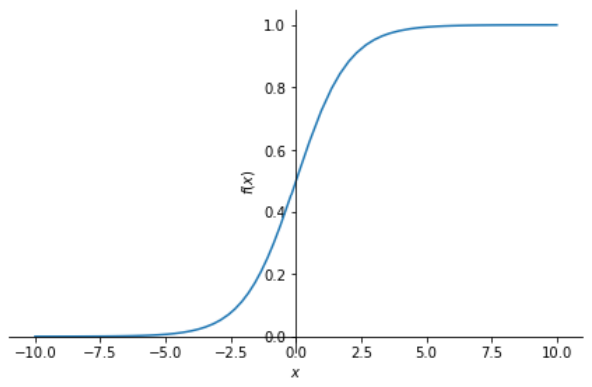
\includegraphics[scale=1]{correcionImgss40.png}
	\caption{Función logística o sigmoide}
	\label{fig:figura700_3}
\end{figure}

Esta función matemática con forma de \textit{S estilizada} presenta un comportamiento asintótico en los valores de 0 y 1, teniendo dicha tendencia para el valor de \textit{f(x)=0} cuando su argumento \textit{x} es negativo, 
y la misma tendencia para \textit{f(x)=1} cuando el argumento es positivo.

%Para esta función su uso convencional está dado por el uso de \textit{$\sigma$}.

A partir de la teoría de modelos probabilísticos para un problema de 2 clases, se sabe que la probabilidad de una clase $C_1$ dado un conjunto de valores de entrada \textbf{x} puede expresarse de la forma (\ref{eq:ecuacion713}) \cite{bishop}.

\begin{equation}
	p(C_1 | \textbf{x})=\sigma ((w)^T \textbf{x})
	\label{eq:ecuacion713}
\end{equation}

Por lo tanto, para la clase restante se tiene (\ref{eq:ecuacion714}).

\begin{equation}
	p(C_2 | \textbf{x})=1-p(C_1 | \textbf{x})
	\label{eq:ecuacion714}
\end{equation}

Las ecuaciones (\ref{eq:ecuacion713}) y (\ref{eq:ecuacion714}) constituyen el modelo de \textit{regresión logística} para clasificación. Para poder ajustar los pesos del modelo mediante técnicas de descenso por gradiente, 
primero se define lo que se conoce como \textit{función de verosimilitud} para la regresión logística (\ref{eq:ecuacion715}), la cual describe la probabilidad de un conjunto de targets dado un cierto valor en los pesos del modelo \cite{bishop}.

\begin{equation}
	p(\textbf{t} | \textbf{w})=\prod_{n=1}^{N} (y_n)^{t_n} (1-y_n)^{1-t_n}
	\label{eq:ecuacion715}
\end{equation}

donde el factor $y_n$ es la probabilidad de una de las clases dado un vector de características de entrada para el clasificador.

A partir de (\ref{eq:ecuacion715}), se puede definir una \textit{función de error} para la regresión logística. Para esto, se debe aplicar el inverso aditivo del logaritmo natural a la función de verosimilitud (\ref{eq:ecuacion716}) \cite{bishop}.

\begin{equation}
	E(\textbf{w})= -ln (p(\textbf{t} | \textbf{w}))  =- \sum_{n=1}^{N} {t_n ln(y_n) + (1 - t_n) ln (1-y_n)}
	\label{eq:ecuacion716}
\end{equation}

Al tomar el gradiente de la función en (\ref{eq:ecuacion716}) con respecto al vector de pesos, se tiene (\ref{eq:ecuacion717}) \cite{bishop}.

\begin{equation}
	\nabla{E(\textbf{w})}= \sum_{n=1}^{N} {(y_n - t_n) x_n}
	\label{eq:ecuacion717}
\end{equation}

Es decir, para este caso particular el gradiente de la fu{nción de costo del algoritmo depende del error del modelo, es decir, la diferencia del valor predicho y el valor real, además del vector de características o datos 
de entrada. Una vez que se tiene el resultado (\ref{eq:ecuacion717}), con él se puede avanzar con el método iterativo para actualizar el vector de pesos del modelo tomando como referencia la información que entrega el 
gradiente de la función de costo. El método para este caso se basa en el algoritmo de \textit{optimización iterativa de Newton-Raphson}, el cual trabaja con aproximaciones cuadráticas para la función de verosimilitud \cite{bishop}. El 
algoritmo de actualización de Newton-Raphson para minimizar una función de costo toma la forma (\ref{eq:ecuacion718}).

\begin{equation}
	{\textbf{w}}_{new}= {\textbf{w}}_{old} -{(\textbf{H})^{-1}} \nabla{E(\textbf{w})}
	\label{eq:ecuacion718}
\end{equation}

donde \textbf{H} es la \textit{matriz Hessiana}, la cual se forma con las segundas derivadas de la función de costo con respecto a las componentes del vector de pesos \textbf{w}, dada por (\ref{eq:ecuacion719}).

\begin{equation}
	\textbf{H}= \nabla{\nabla{E(\textbf{w})}}
	\label{eq:ecuacion719}
\end{equation}

Por lo tanto, la ecuación para la actualización iterativa de los pesos del modelo de regresión logística queda de la forma (\ref{eq:ecuacion720}).

\begin{equation}
	{\textbf{w}}_{new}= {\textbf{w}}_{old} -{(\nabla{\nabla{E(\textbf{w})}})^{-1}} \nabla{E(\textbf{w})}
	\label{eq:ecuacion720}
\end{equation}

El método de regresión logística al tener un enfoque probabilístico, de manera general los resultados entregados por la función sigmoide para un conjunto de pesos y valores de entrada específicos, son valores que representan 
las probabilidades para cada una de las clases involucradas. Es decir, al evaluar el modelo se tienen como resultados valores entre 0 y 1 para cada clase individual, indicando estos la probabilidad correspondiente a cada 
clase de ser la estimación correcta. Igualmente, la suma de los valores dados como resultado debe ser 1, y la estimación para el modelo suele determinarse tomando como referencia el resultado de magnitud mayor, entendiéndose 
que la clase correspondiente a dicho resultado es la estimación dada por este método.

\section{Redes Neuronales Artificiales}

\subsection{La Neurona Biológica}

El concepto o idea de Neurona fue introducido a finales del siglo XIX por el científico español Santiago Ramón y Cajal. En sus investigaciones planteó que el sistema nervioso del cuerpo humano estaba compuesto por neuronas 
individuales, las cuales se comunicaban entre sí por medio de interacciones a las que denominó \textit{sinápsis} \cite{caicedoANN}. Actualmente, gracias al desarrollo de la neurobiología sabemos que este planteamiento es 
válido.

Básicamente, una neurona es un tipo de célula biológica. Su forma esférica varía entre 5 a 10 micras de diámetro, y de ella emanan una rama principal denominada \textit{axón}, además de otras ramas de longitud más corta 
denominadas \textit{dendritas} \cite{caicedoANN}. En la \autoref{fig:figura700_4} se muestra una ilustración de la estructura de una neurona biológica.

\begin{figure}[h]
	\centering
	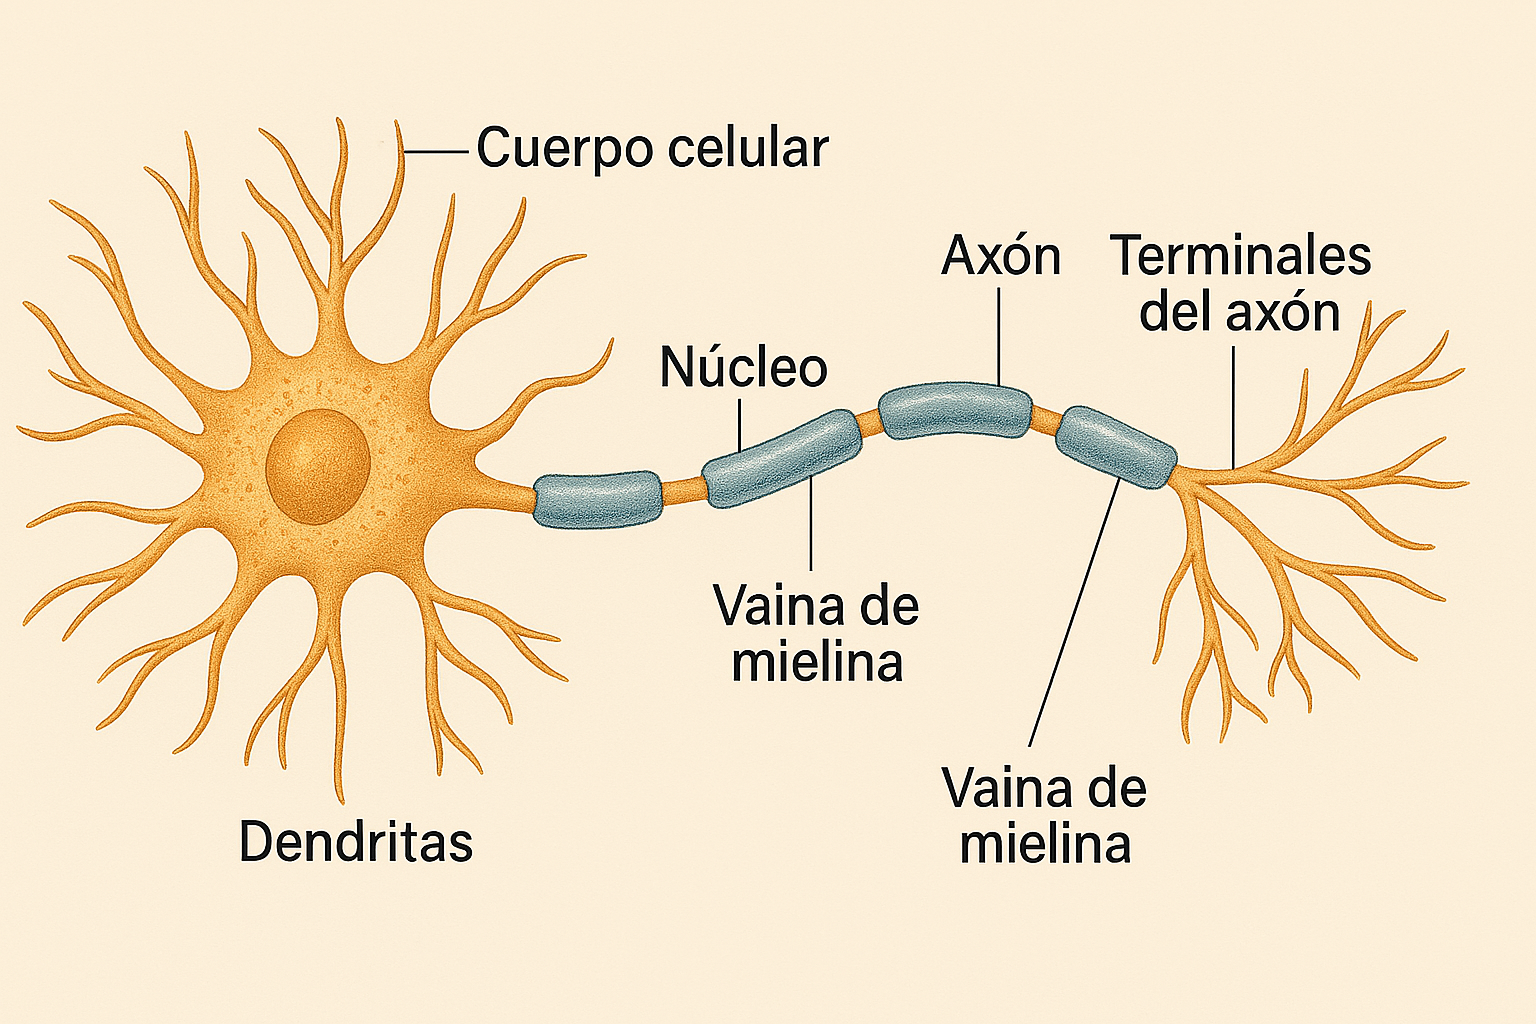
\includegraphics[scale=0.2]{imgss214.png}
	\caption{Estructura básica de una neurona biológica. Imagen generada con recursos de Internet}
	\label{fig:figura700_4}
\end{figure}

Una de las características que diferencian a las neuronas de otros tipos de células biológicas, es la capacidad que tienen para comunicarse. Este proceso de comunicación consiste en que las dendritas y el cuerpo de la neurona 
reciben señales de entrada, las cuales el cuerpo de la neurona las combina y posteriormente se emiten señales de salida a través de la terminal del axón, el cual se encarga de transmitir dicha salida a un nuevo conjunto de
neuronas. Generalmente, una neurona recibe información de miles de otras neuronas y envía información a miles de otras más \cite{caicedoANN}.

En una neurona, las señales existentes puedes ser de naturaleza química o eléctrica; la señal generada por la neurona y transportada mediante el axón es una señal eléctrica, mientras que la señal que se transmite entre la 
terminal del axón y las dendritas de otras neuronas es una señal de naturaleza química. La comunicación entre neuronas no se realiza mediante contacto directo, se lleva a cabo a través del fenómeno denominado \textit{sinápsis}.
La sinápsis es un espacio que está ocupado por unas sustancias químicas llamadas neurotransmisores, los cuales se encargan de bloquear o dejar pasar las señales que provienen de otras neuronas. En este punto, una neurona 
dada va recibiendo las señales provenientes de otras neuronas con las que tenga comunicación, y dichas señales se acumulan para posteriormente definir qué hacer \cite{caicedoANN}.

Cuando se tiene la acumulación de un conjunto de señales, si la \textit{suma} de todas ellas es lo suficientemente grande, se puede vencer el \textit{potencial de acción}, lo que permite que la neurona se active o por el 
contrario permanezca inactiva. Si la neurona es capaz de activarse, entonces tiene la capacidad de transmitir un impulso eléctrico a las neuronas con las cuales tiene comunicación, las cuales reciben dicho impulso como una 
entrada \cite{caicedoANN}.

\subsection{Aproximación Matemática Para Un Modelo De Neurona Artificial}

La \autoref{fig:figura700_5} muestra un dibujo para explicar el proceso de cómo sería una formulación matemática para llevar la neurona biológica a un modelo matemático que después pueda ser de utilidad para las Redes Neuronales 
Artificiales. Comúnmente este modelo se le denomina \textit{perceptrón}.

\begin{figure}[h]
	\centering
	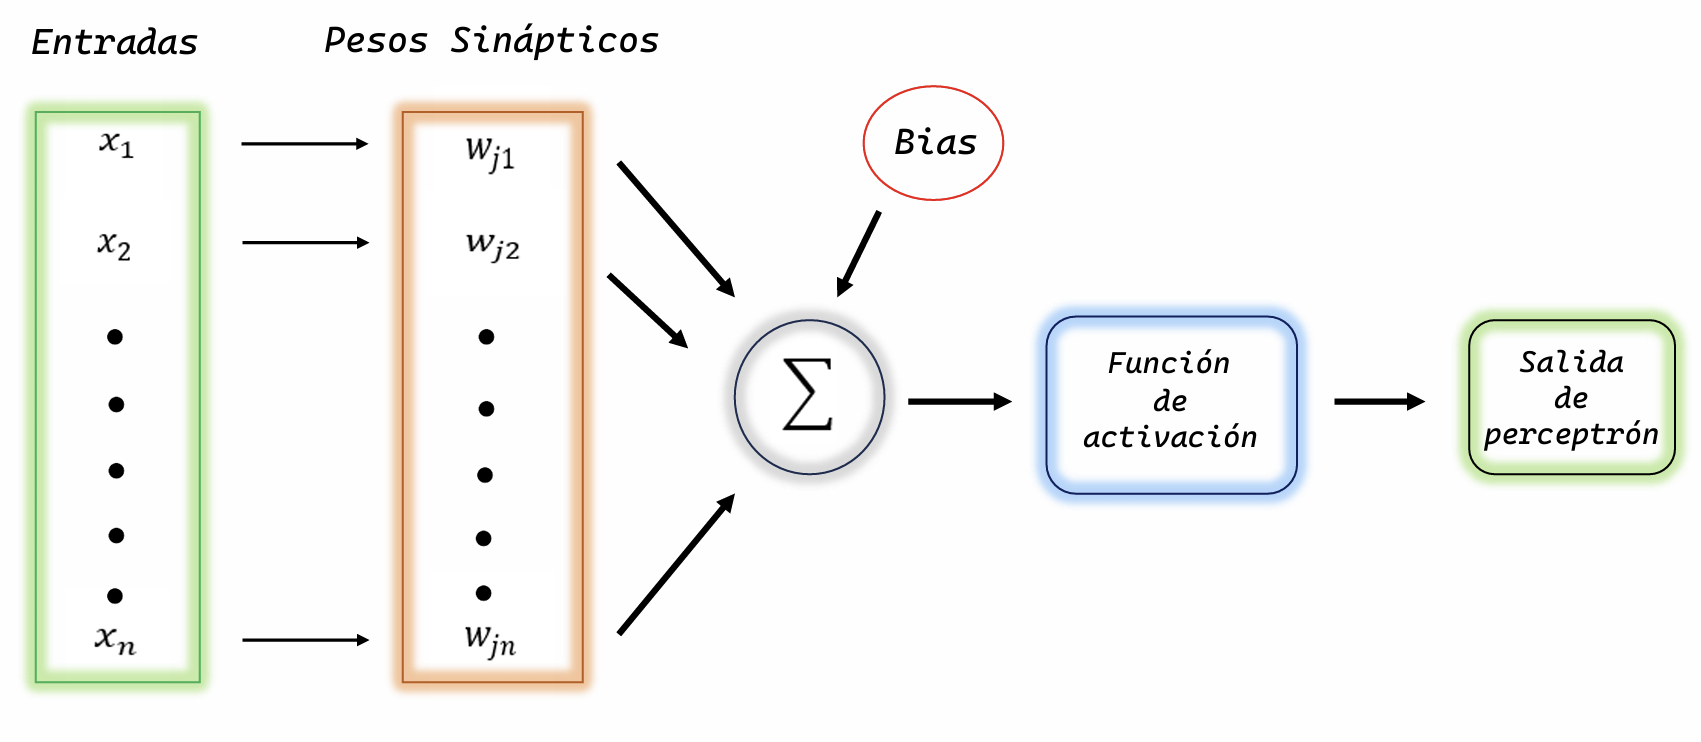
\includegraphics[scale=0.55]{imgss219.png}
	\caption{Modelo de perceptrón}
	\label{fig:figura700_5}
\end{figure}

Al igual que una neurona biológica, para el modelo de perceptrón también se tienen las entradas receptoras de señales provenientes de otras neuronas con las cuales hay conexión para transmisión de información \cite{caicedoANN}. 
Para el modelo planteado en la \autoref{fig:figura700_5}, el vector de entradas \textbf{X} toma la forma (\ref{eq:ecuacion721}).

\begin{equation}
	\textbf{X}= (x_1, x_2, ... , x_n)
	\label{eq:ecuacion721}
\end{equation}

La información recibida en la neurona es modificada por un vector de \textit{pesos sinápticos} \textbf{W}, cuyo papel es emular la sinápsis existente entre las neuronas biológicas. Estos valores de pesos sinápticos se pueden 
interpretar como una \textit{ganancia en la señal}, es decir, amplificar o atenuar los valores de entrada. Adicionalmente, se coloca un término constante conocido como \textit{bias o sesgo}, cuya función es agregar una señal 
adicional a la \textit{función de activación} con el propósito de eliminar la linealidad del modelo provocada cuando las entradas son iguales a 0 \cite{caicedoANN}.

Los diferentes valores que recibe la neurona a las entradas, modificados por los pesos, son sumados para generar el resultado \textit{entrada neta}, la cual es la que determinará si la neurona artificial se activa o no lo hace. 
La activación de la neurona dependerá de la \textit{función de activación} elegida para cada caso específico, ya que existen diferentes funciones de activación, cada una con ventajas y desventajas dependiendo de la aplicación 
que tenga el modelo \cite{caicedoANN}. La ecuación (\ref{eq:ecuacion722}) representa el resultado de entrada neta para este modelo:

\begin{equation}
	Net_j= \sum_{i=1}^{n} {x_i w_{ji} + Bias_j}
	\label{eq:ecuacion722}
\end{equation}

donde el subíndice \textit{i} corresponde al i-ésimo dato de entrada al modelo. El subíndice \textit{j} hace referencia a que este tipo de modelo se puede extender a un modelo con un mayor número de capas verticales de neuronas 
apiladas, por lo tanto el subíndice \textit{j} haría referencia a la j-ésima capa en un modelo extendido. La expresión anterior también se puede expresar usando multiplicación matricial de la forma (\ref{eq:ecuacion10722}):

\begin{equation}
	Net_j=(\textbf{w})^{T} \textbf{x} + Bias_j
	\label{eq:ecuacion10722}
\end{equation}

El vector \textbf{w} dado por la expresión anterior puede expresarse de una forma general usando la ecuación (\ref{eq:ecuacion10726}):

\begin{equation}
	\textbf{w}=(w_{j1}, w_{j2}, ... , w_{jn})
	\label{eq:ecuacion10726}
\end{equation}

La salida de la neurona artificial está determinada por la función de activación \textit{f} de la forma (\ref{eq:ecuacion723}).

\begin{equation}
	y_j= f(Net_j)
	\label{eq:ecuacion723}
\end{equation}

El modelo individual de 1 sola neurona artificial representa una herramienta con baja capacidad de procesamiento, por lo cual su nivel de aplicabilidad en la solución de problemas reales es bajo. Su verdadero potencial radica 
cuando se realiza la interconexión de un gran número de neuronas individuales, tal y como ocurre por ejemplo en el cerebro humano. Esto es lo que conduce al concepto de Red Neuronal Artificial; un modelo de esta naturaleza 
compuesto por una gran cantidad de elementos simples (neuronas o nodos) de procesamiento, los cuales tienen la capacidad de operar en paralelo, y cuyo propósito o función es determinado por la estructura o \textit{arquitectura}
de la red neuronal, así como también por el ajuste u optimización realizado sobre los valores de los pesos sinápticos que servirán como intermediarios en la comunicación entre nodos o neuronas individuales \cite{caicedoANN}.

\subsection{Interconexión De Neuronas Para Una Red Neuronal Artificial}

La \autoref{fig:figura700_6} muestra un diagrama de una red neuronal conformada por varias neuronas o \textit{nodos} distribuidos en 3 \textit{capas}.

\begin{figure}[h]
	\centering
	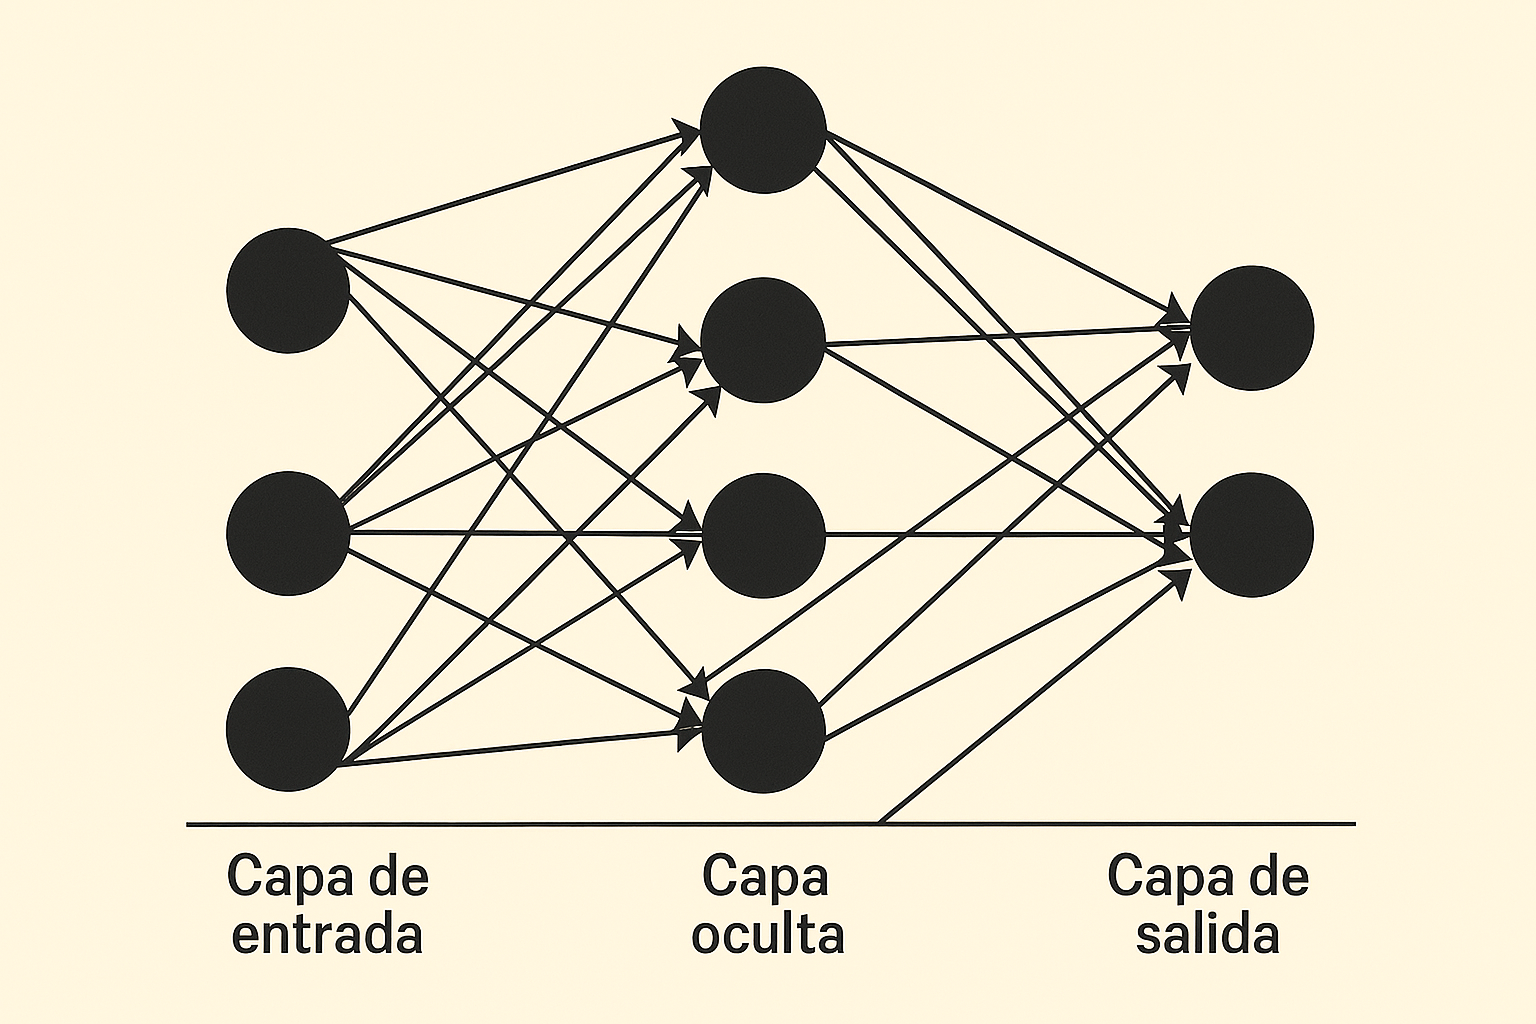
\includegraphics[scale=0.25]{imgss215.png}
	\caption{Diagrama de modelo de red neuronal artificial. Imagen generada con recursos de Internet}
	\label{fig:figura700_6}
\end{figure}

El ejemplo mostrado en la \autoref{fig:figura700_6} es un ejemplo básico en cuanto a tamaño de la red, pero suficiente para explicar en qué consiste y cómo se ampliaría a una arquitectura más general.

Cada uno de los puntos de color negro corresponde a una neurona o nodo, y cada uno de ellos mantiene una conexión con otras neuronas, tanto previas como posteriores. Toda Red Neuronal está compuesta por \textbf{\textit{capas}},
que son cada una de las columnas de nodos, en nuestro caso tenemos 3 capas. Dentro de esta característica, igualmente en cualquier Red Neuronal encontraremos 3 tipos de capas: la \textbf{\textit{capa de entrada o input layer}},
\textbf{\textit{capas ocultas o hidden layers}} y \textbf{\textit{capa de salida o output layer}} \cite{deitelIA}. 

La capa de entrada es siempre la columna de nodos que se encuentra más a la izquierda en el diagrama; en ella se colocan tantos nodos como número de variables de entrada con las que se va a trabajar. La capa de salida es siempre la columna de neuronas que se encuentra más a la derecha del diagrama; el número de nodos a colocar en esta capa es igual al número de variables de salida que se requieren. 

Por ejemplo, si la Red Neuronal va a trabajar como un algoritmo de regresión, únicamente se colocará un nodo en la capa de salida, el cual corresponderá a la variable target que se 
busca predecir. Si la Red Neuronal se planteará para usarse como algoritmo de clasificación, el número de nodos en la capa de salida sería igual al número de clases posibles en el problema de clasificación que se busca resolver.

Finalmente, las capas ocultas son todas las columnas de nodos que se encuentren entre la capa de entrada y la capa de salida; en nuestro ejemplo solo se muestra 1 capa oculta, pero se pueden colocar las que sean necesarias 
de acuerdo a las necesidades del problema a resolver. Referente al número de nodos en cada capa oculta, igualmente se pueden colocar la cantidad que sea necesaria acorde al propósito que tenga la Red Neuronal \cite{AurelienGeron}. 

Es necesario aclarar que mientras mayor sea el número de capas ocultas y nodos en cada una de ella, el modelo matemático generado será mucho más complejo y más difícil de procesar a nivel de cálculo computacional, pero es 
precisamente el generar una Red de mayor tamaño lo que permite resolver problemas más complejos, es decir, una Red Neuronal con 1 capa oculta y 20 nodos en ella tendrá menor capacidad de aprendizaje
para resolver un problema de alta complejidad que una Red con 10 capas ocultas y 50 nodos en cada una de ellas.

En la \autoref{fig:figura700_6}, también se muestran las conexiones existentes entre las neuronas de diferentes capas, teniendo en este caso que cada neurona de la capa de entrada se conecta a todas las neuronas de la capa 
oculta; las neuronas de la capa oculta se conectan a todas las neuronas de la capa previa y la capa posterior, ya sea que la capa posterior sea otra capa oculta o la capa de salida y la capa previa sea la capa de entrada u 
otra capa oculta. 

La conexión entre 2 neuronas cualesquiera está definida siempre por un peso sináptico, los cuales servirán como coeficientes para una combinación lineal de todas las entradas a una neurona específica, y dicha combinación 
lineal será la entrada para la función de activación de cada neurona. Es decir, por ejemplo para la \autoref{fig:figura700_6}, a cada una de las neuronas de la capa oculta su entrada es la combinación lineal de las señales
provenientes de la capa de entrada, y las neuronas de la capa oculta evaluan esa combinación mediante su función de activación, la cual emite una señal de salida. Por lo tanto, de la capa oculta se tendrán 4 señales de 
salida, cada una proveniente de nodos distintos, y estas señales ahora serán las que servirán para formar combinaciones lineales que serán las entradas a las neuronas de la capa de salida, las cuales nuevamente evalúan las
combinaciones mediante sus funciones de activación para poder entregar señales de salida, las cuales en este caso ya serían el resultado final.

Por último, tanto en las capas ocultas como en la capa de salida, otro elemento importante es el término individual de \textit{bias} o \textit{sesgo} que corresponde a cada una de estas capas en la red; estos términos son 
valores numéricos constantes de inicio y que pueden modificar sus valores también cuando se realiza la optimización de los pesos sinápticos durante el entrenamiento de la red. De forma matemática, cada uno de estos términos 
se convierte en otro elemento o término adicional para cada una de las combinaciones lineales formadas para cada nodo de las capas ocultas y capa de salida.

La principal función de los terminos bias es evitar que los nodos de una red neuronal emitan una señal de salida de 0 cuando los valores de entrada son 0 para ese conjunto específico de nodos en el modelo. Esto evita que 
se anulen o hagan 0 los valores propagados hacia adelante a través de la red, además de que estos términos bias ayudan a generar patrones matemáticos o geométricos más complejos, lo que hace al modelo tener mejores resultados.

\subsection{Funciones De Activación}

En una Red Neuronal es posible tener 1 sola función de activación en todas las capas, o por ejemplo una función específica para las capas ocultas y otra función diferente para los nodos de la capa de salida. Todo dependerá 
del tipo de aplicación que va a desarrollar el modelo. A continuación se describen las funciones más comunes.

\textbf{\textit{Función ReLU (Rectified Linear Unit, Unidad Rectificada Lineal)}}. Se define de la forma (\ref{eq:ecuacion724}).

\begin{equation}
	f(x)=\textbf{max} (0,x)
	\label{eq:ecuacion724}
\end{equation}

Su gráfica se muestra en la \autoref{fig:figura700_7}.

\begin{figure}[h]
	\centering
	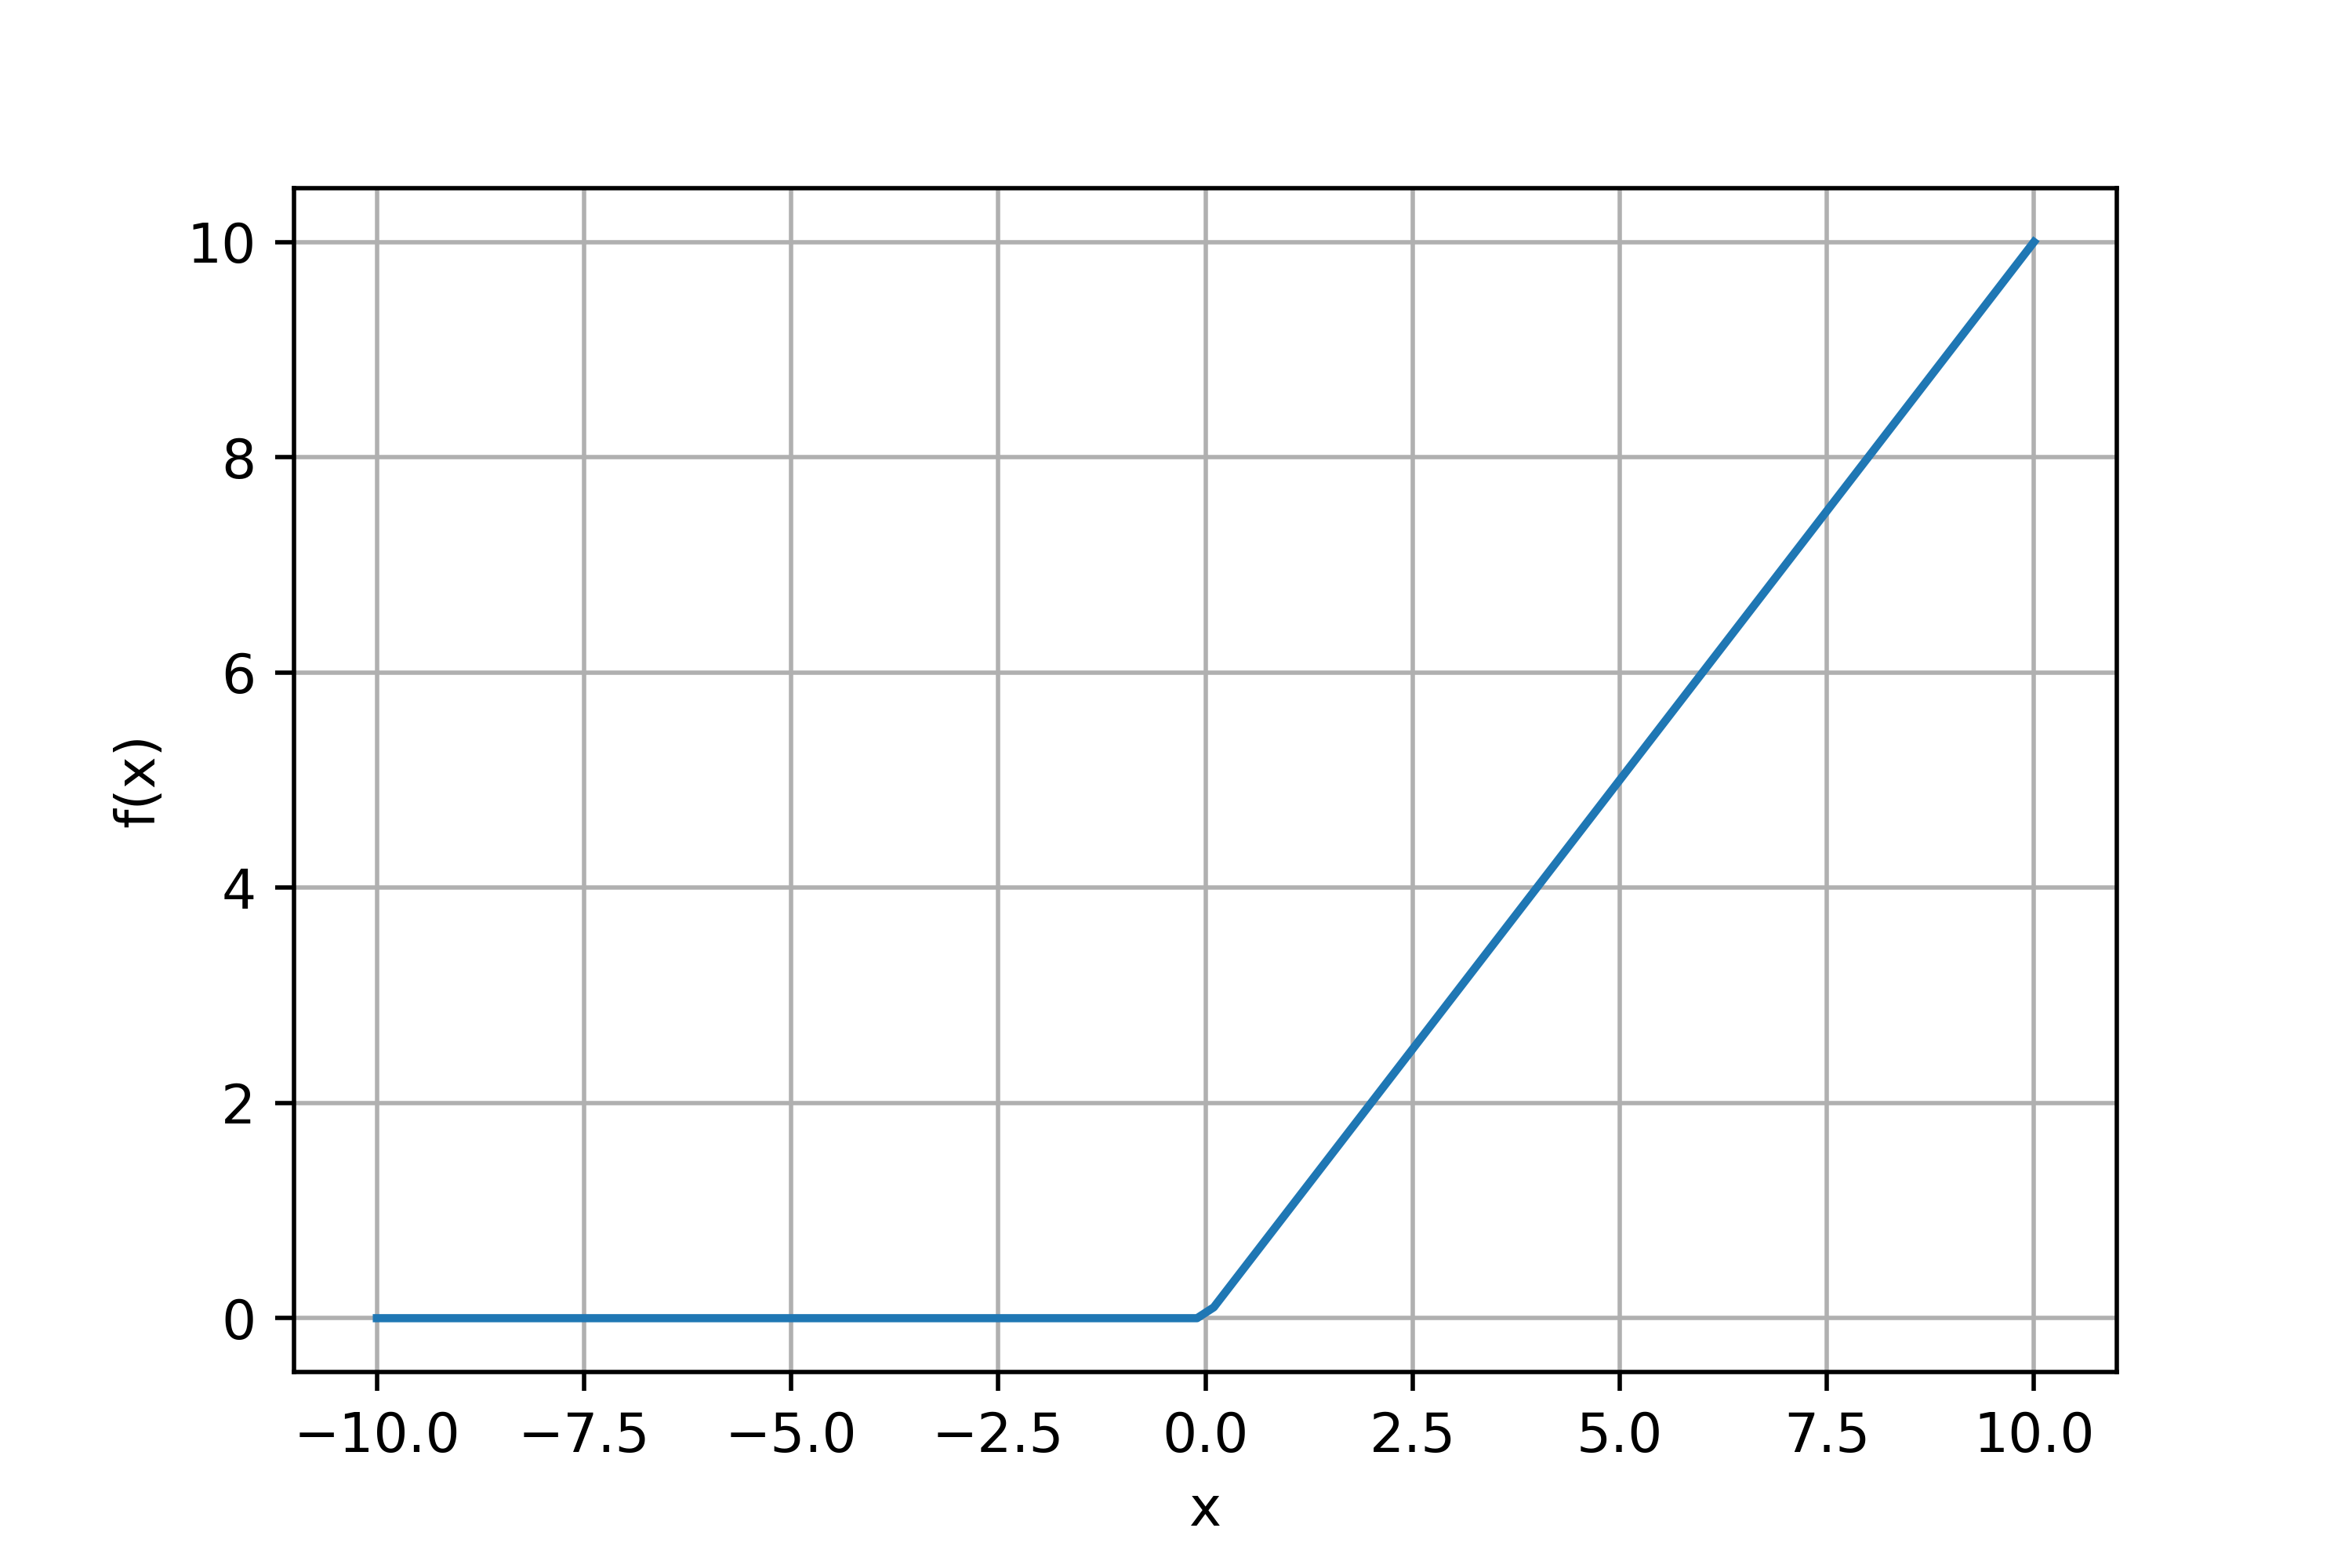
\includegraphics[scale=0.8]{imgss149.png}
	\caption{Función ReLU}
	\label{fig:figura700_7}
\end{figure}

Se trata de una función de tipo rampa, la cual al ser negativa la variable de entrada, la salida entregada es 0; si la entrada a la función es positiva, entonces el valor a la salida es igual al valor a la entrada. Dado 
lo anterior, en una red neuronal esta función permite eliminar cualquier valor negativo generado por las ecuaciones implícitas en el algoritmo \cite{ReluBarcelona}.

Entre las ventajas que ofrece están la de acelerar la convergencia del algoritmo de optimización de descenso por gradiente para casos específicos en comparación con otras funciones de activación diferentes, además de que 
su implementación en código resulta muy simple. Una desventaja importante que posee tiene que ver con el hecho de que es una función que puede llegar a \textit{morir}, es decir, que durante el proceso de optimización de 
los pesos de la red, se llegue a una circunstancia donde dicha función nunca vuelva a dispararse, siendo 0 su salida sin posibilidad de revertir este efecto \cite{ReluBarcelona}.

\textbf{\textit{Función sigmoide}}. Se define de la forma (\ref{eq:ecuacion725}).

\begin{equation}
	\sigma(x)=\frac{1}{1+exp(-x)}
	\label{eq:ecuacion725}
\end{equation}

Su gráfica se muestra en la \autoref{fig:figura700_8}.

\begin{figure}[h]
	\centering
	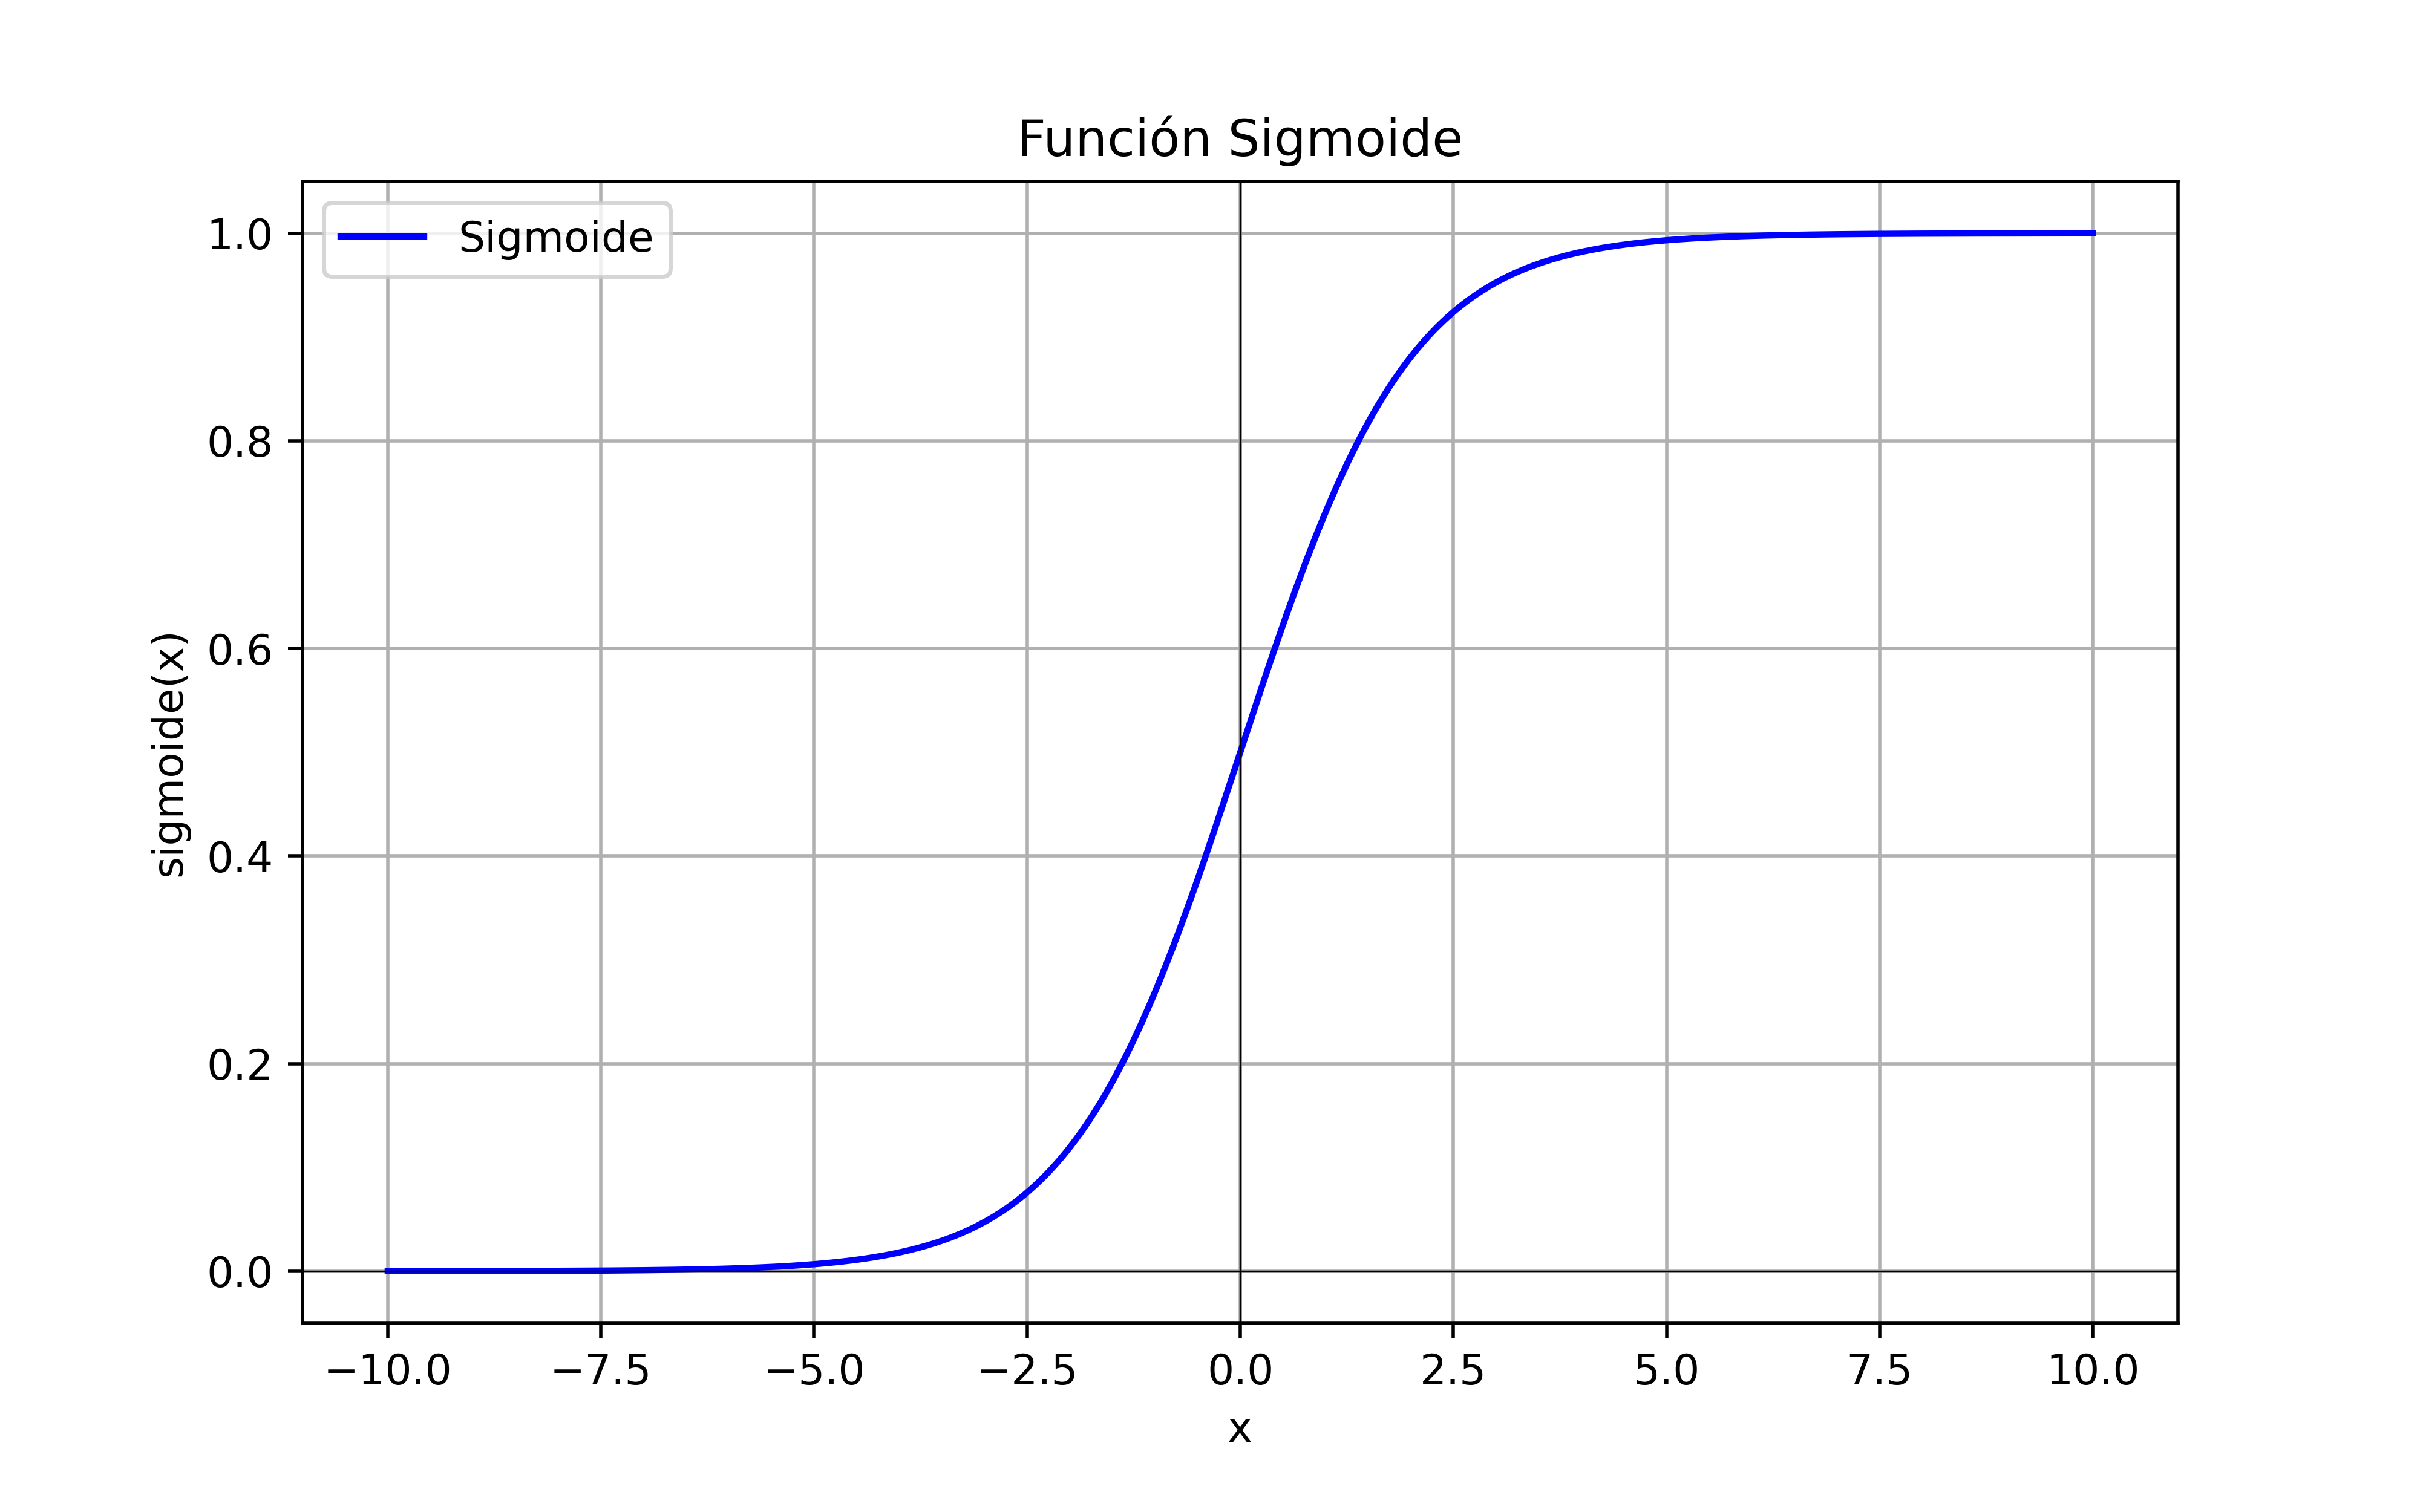
\includegraphics[scale=0.8]{imgss205.png}
	\caption{Función Sigmoide}
	\label{fig:figura700_8}
\end{figure}

Es una función de tipo exponencial que para valores cercanos a 0 en la variable de entrada, cambia de forma acelerada su valor de salida de un valor muy cercano a 0 a un valor muy cercano a 1 y viseversa. 
Indicando también que para un valor de entrada de \textit{x=0}, la función toma 0.5 como valor.
Para valores negativos a la entrada, la función tiene un comportamiento asintótico sobre el valor de 0, y para valores positivos de entrada la función tiene también un comportamiento asintótico, pero ahora sobre el valor de 1 \cite{SeriesTemporalesAvanzadas}.

Entre sus propiedades, permite que en la Red Neuronal se tengan valores de salida de cada una de las capas en un rango de 0 a 1, logrando así no tener valores que se disparen a magnitudes elevadas, sobre todo cuando los 
rangos de valores de las variables de entrada a la Red son muy distintos. Una razón por la cual también es importante hacer un escalamiento de los valores de entrada a la Red cuando se usa esta función \cite{RNAlineasDeTransmisión}. 

Adicionalmente, facilita las aplicaciones destinadas a problemas de clasificación binaria, es decir, únicamente 2 clases posibles. Esto se logra debido a que se aprovecha la propiedad de la función de que conmuta entre 0 
y 1 \cite{RNAlineasDeTransmisión}. 

\textbf{\textit{Tanh (Función Tangente Hiperbólica)}}. Se define de la forma (\ref{eq:ecuacion726}):

\begin{equation}
	tanh(x)=\frac{exp(x) - exp(-x)}{exp(x) + exp(-x)}
	\label{eq:ecuacion726}
\end{equation}

Su gráfica se muestra en la \autoref{fig:figura700_9}.

\begin{figure}[h]
	\centering
	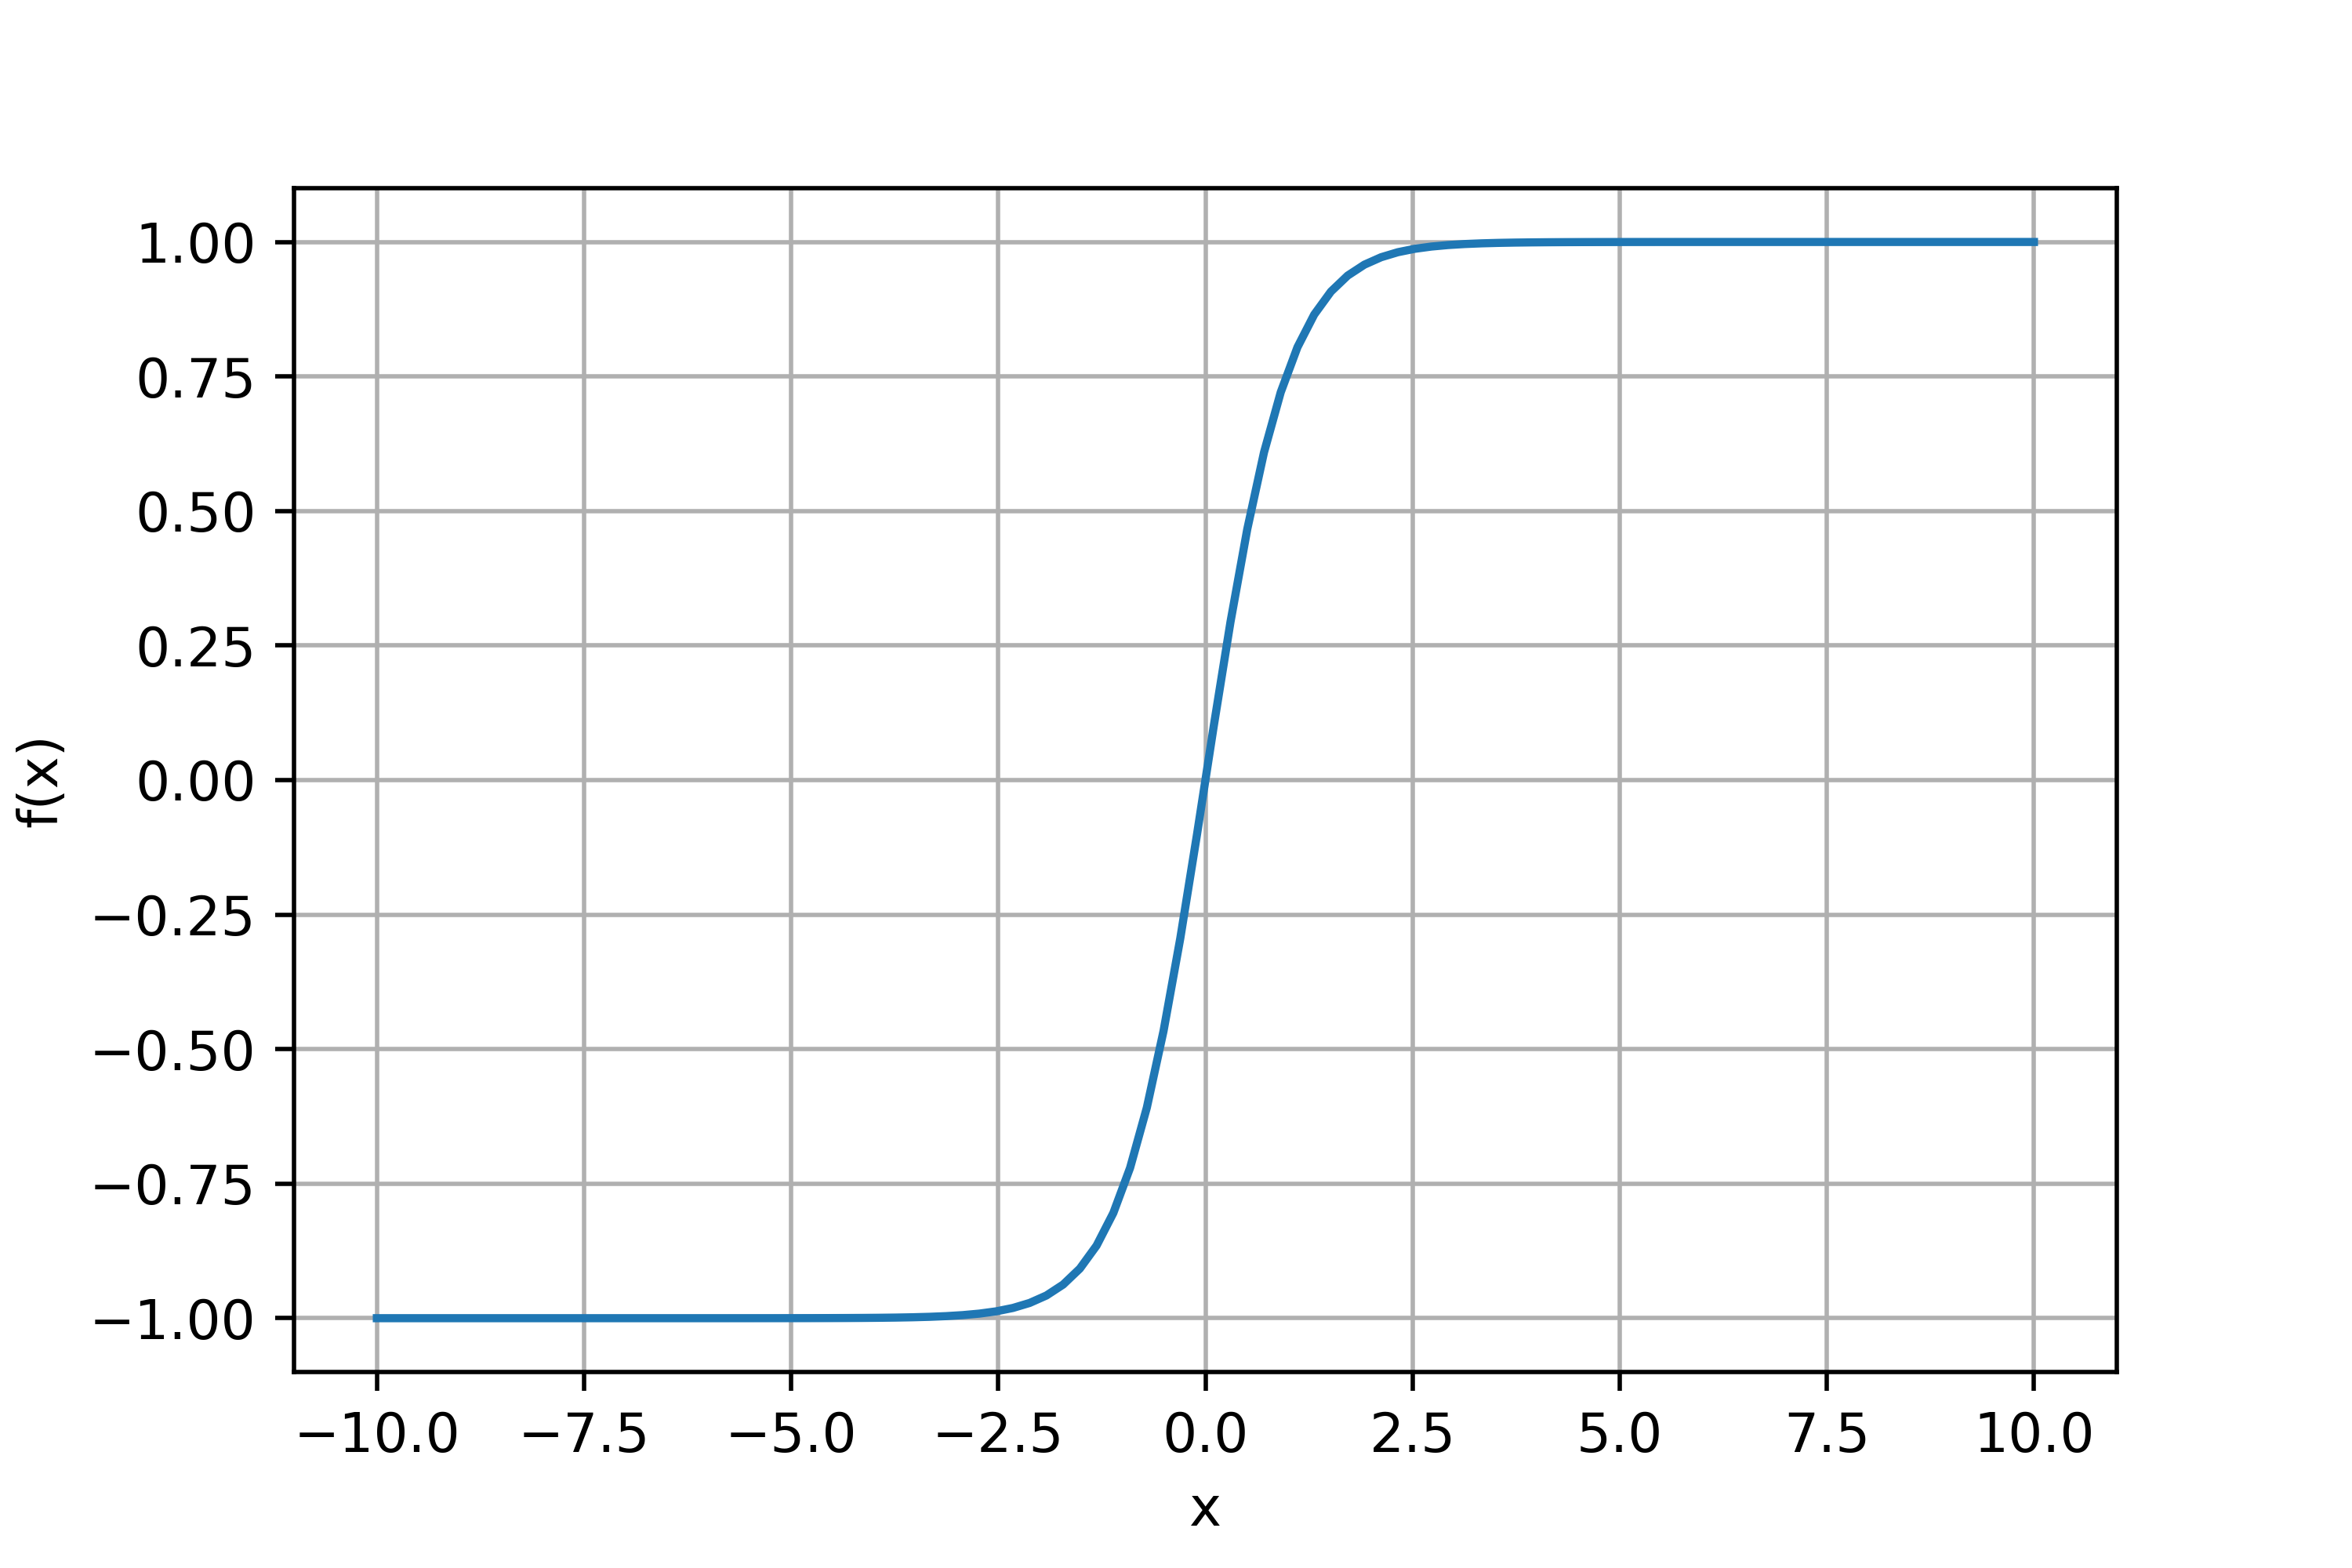
\includegraphics[scale=0.8]{imgss150.png}
	\caption{Función tangente hiperbólica}
	\label{fig:figura700_9}
\end{figure}

En la \autoref{fig:figura700_9} se observa que tiene la misma forma que la función sigmoide, sin embargo, para valores negativos de la variable de entrada ahora el comportamiento asintótico es sobre el valor de -1, y la 
función sigmoide lo hace sobre el valor de 0. Esta diferencia es precisamente un factor importante para elegirla en vez de a la sigmoide, debido a que su rango de valores de salida no se corta en 0, sino que permite también 
entregar valores negativos como señal de salida. 

Otras ventajas que tiene sobre la sigmoide es que suele acelerar la convergencia en la optimización de los pesos sinápticos durante el ajuste del modelo, además de que disminuye 
el efecto de desvanecimiento del gradiente, es decir, que durante el ajuste de la red se generen valores que tiendan a 0, lo cual provoca generalmente que el entrenamiento se vuelva muy lento, es decir, que llegue a 
requerir un número muy grande de iteraciones. En el caso de la aceleración en la convergencia en el entrenamiento de una red neuronal al usar la función tangente hiperbólica, este efecto se debe principalmente a que la sigmoide 
solo tiene salidas con valores positivos, mientras que la función tangente hiperbólica admite salidas con valor negativo lo que permite tener más estabilidad en la magnitud de los \textit{saltos} dados en el proceso de descenso 
por gradiente \cite{RNAconceptosBasicos}.

\textbf{\textit{Función Softmax}}. Se define de la forma (\ref{eq:ecuacion727}).

\begin{equation}
	f(x)_j=\frac{exp(x_j)}{\sum_{i=1}^{K} {exp(x_i)}}
	\label{eq:ecuacion727}
\end{equation}

El factor \textit{K} es el número de clases posibles en el clasificador; el subíndice \textit{j} hace referencia a la j-ésima clase.

La función softmax usualmente es aplicable en problemas de clasificación, ya que permite calcular la probabilidad de cada clase sobre todas las clases posibles, factor que la convierte en una opción efectiva para casos de 
clasificación multiclase. Una función con esta forma se puede aprovechar para colocarse en los nodos de la capa de salida de una Red Neuronal, debido a que entregará como resultado un rango de probabilidad de salida entre 
0 y 1, teniendo que la suma de todas las probabilidades dará un resultado de 1 \cite{tanhArgentina}.

\textbf{\textit{Función Lineal}}. Se define de la forma (\ref{eq:ecuacion728}).

\begin{equation}
	f(x)=x
	\label{eq:ecuacion728}
\end{equation}

Lo que nos dice la ecuación (\ref{eq:ecuacion728}) es que la salida entregada por esta función es igual a la señal que recibe a la entrada.

El caso más significativo de uso de esta función es en la capa de salida en problemas de regresión. Esto es debido a que en este tipo de problemas se busca predecir una valor numérico target único, por lo tanto al usar esta 
función se asegura que el modelo entregará un resultado numérico al que no se le halla aplicado ninguna transformación matemática \cite{RNAconceptosBasicos}.

En el caso contrario, en las capas ocultas de una Red Neuronal no es recomendable el uso de la función lineal debido a que lo que se busca en las capas ocultas es generar patrones no lineales complejos, que son precisamente 
los que permiten abordar con éxito la mayoría de las aplicaciones \cite{RNAconceptosBasicos}.

\subsection{Entrenamiento De Una Red Neuronal}

Sea cual sea el propósito que se le dé a una Red Neuronal, ya se ha mencionado que el modelo debe optimizarse o entrenarse para poder llegar a la mejor aproximación posible en el conjunto de pesos sinápticos que forman parte 
del modelo. Dicho entrenamiento requiere \textbf{\textit{datos}}, pero de dónde deben surgir o conseguirse; todo depende del problema que se quiera resolver. Si el modelo se usará para procesamiento de audio, entonces los 
datos deben recolectarse de señales de audio; si se busca hacer procesamiento de imagen, consecuentemente los datos deben provenir de imágenes.

La idea es que para el propósito que tenga la Red Neuronal, se requiere obtener la mayor cantidad de información posible acerca del fenómeno, proceso o procedimiento en donde se busca trabajar con el algoritmo; se necesita 
establecer un conjunto de variables o parámetros característicos de los cuales obtener la mayor cantidad de valores posibles de cada uno de ellos, y dicha información formará el conjunto de datos que nos permitirá aplicar 
una metodología conocida como \textbf{\textit{Feed-Forward o Propagación Hacia Adelante}}. 

Una vez que se ha recolectado toda la información para el conjunto de datos o \textit{dataset} para el modelo, es necesario dividirlo en 2 subconjuntos; el primero, para el entrenamiento del modelo, y el segundo para realizar 
la \textit{validación} del modelo, es decir, verificar qué tan bien el modelo es capaz de entregar los resultados requeridos. Dicha fragmentación del dataset generalmente suele realizarse asignando el 80$\%$ de todos los 
datos para entrenamiento y el 20$\%$ restante para validación; otra convención también usada ampliamente es asignar el 70$\%$ de los datos para entrenamiento y el 30$\%$ restante para validación \cite{caicedoANN}.

Aparte del método Feed-Forward ya mencionado, el segundo procedimiento a ejecutar para lograr el ajuste de la Red Neuronal es el método de \textbf{\textit{Error Backpropagation, Propagación Hacia Atrás del Error}}. La aplicación
de estos 2 métodos nos permitirá obtener información sobre el estado de la Red Neuronal durante el entrenamiento, lo cual finalmente nos permitirá aplicar el algoritmo de descenso por gradiente para minimización de la función 
de costo.

La aplicación del método Feed-Forward consiste en propagar los datos de entrenamiento de izquierda a derecha a través de la Red Neuronal, es decir, primeramente se tiene la capa de entrada que no aplica función de activación 
alguna. Posteriormente los datos deben propagarse de forma distribuida a través de todos los nodos de todas las capas ocultas. Finalmente,
las señales de salida de la última capa oculta son entrada para la capa de salida, la cual se encarga de entregar el resultado final.

Lo descrito en el párrafo anterior se debe realizar de forma iterativa con todos los datos de entrenamiento disponibles, pero entre cada iteración individual es necesario realizar un ajuste de todos los pesos del modelo tomando 
como referencia el error puntual que se tiene en la salida de la red para cada target. Es en esta parte donde se requiere trabajar con una función de costo o error, la cual sea una función 
matemática que tenga como variables independientes al conjunto de pesos del modelo, y con la cual se pueda trabajar el algoritmo de descenso por gradiente para buscar un valor mínimo global del error y al mismo tiempo encontrar 
la mejor optimización de los pesos sinápticos \cite{BobadillaML}. 

Dado que el error dado en la capa de salida se utiliza como referencia para determinar el nivel de optimización de los pesos en las capas anteriores, es por esta razón que se 
denomina como Propagación Hacia Atrás del Error, ya que el error dado en la salida de la Red Neuronal se distribuye hacia atrás hacia todas las conexiones sinápticas del modelo, y de esta forma poder determinar la 
cantidad de cambio que se aplicará a cada peso en cada iteración durante el proceso de entrenamiento \cite{BobadillaML}.

Una red neuronal consiste en generar funciones no lineales de combinaciones lineales de las entradas. Primeramente, para la capa de entrada si se tiene un conjunto \textit{$x_1$, $x_2$, ... , $x_D$} como variables para el 
modelo, entonces se pueden definir \textit{M} combinaciones lineales de las entradas de la forma (\ref{eq:ecuacion729}).

\begin{equation}
	a_j=\sum_{i=1}^{D} {w_{ji} x_i + w_{j0}}
	\label{eq:ecuacion729}
\end{equation}

donde \textit{j=1,2,...,M} se refieren al número de nodos existentes en la capa siguiente. En la ecuación (\ref{eq:ecuacion729}) también es importante señalar al segundo término en el lado derecho de la ecuación, el cual viene siendo 
el término \textit{bias} para cada uno de los nodos de la capa oculta. El subíndice \textit{i} hace referencia al i-ésimo dato de entrada a la red neuronal; el elemento \textit{$a_j$} es la combinación lineal de entrada 
al j-ésimo nodo de la capa siguiente y \textit{D} es el número total de datos de entrada a la red \cite{bishop}. 

En la \autoref{fig:figura700_200} se muestra un diagrama que ejemplifica lo anteriormente descrito.

\clearpage

\begin{figure}[h]
\centering
  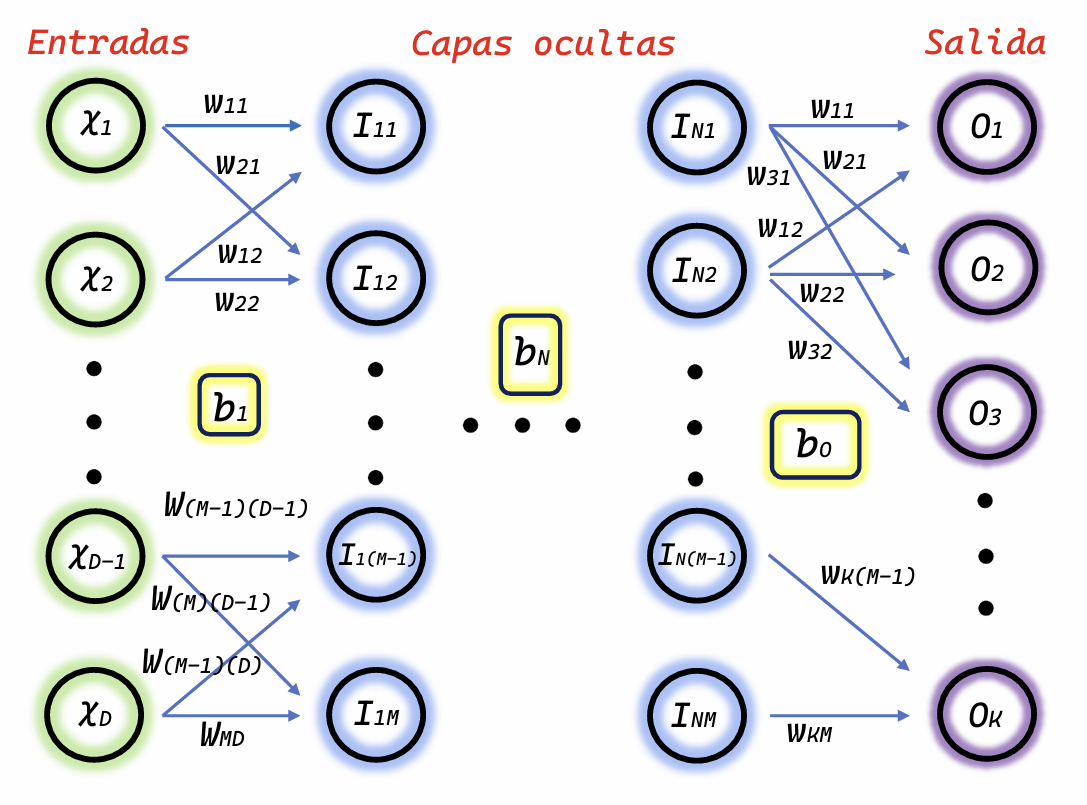
\includegraphics[scale=0.8]{imgss222.png}
  \caption{Representación general de red neuronal}
  \label{fig:figura700_200}
\end{figure}

La \autoref{fig:figura700_200} muestra una representación general con una capa de entrada compuesta por \textit{D} elementos, un número \textit{N} de capas ocultas, cada una de ellas con \textit{M} nodos; en la capa de salida 
se muestra un número \textit{K} de nodos. Adicionalmente, se muestran los términos \textit{$b_1$}, \textit{$b_N$} y \textit{$b_O$}, que son los términos bias correspondientes a capas ocultas y capa de salida, respectivamente. 

Ahora, cada uno de los términos \textit{$a_j$} son transformados usando una función de activación \textit{h} de la forma (\ref{eq:ecuacion730}).

\begin{equation}
	z_j=h(a_j)
	\label{eq:ecuacion730}
\end{equation}

Como ya se explicó en la Sección 2.4.4, se pueden escoger diferentes funciones de activación dependiendo del tipo de problema que se busca resolver. Ahora, los resultados dados por la ecuación (\ref{eq:ecuacion730}) serán 
las entradas para la siguiente capa de la red, que puede ser la capa de salida u otra capa oculta. Si el modelo solo consta de una capa oculta, se tiene la ecuación (\ref{eq:ecuacion731}), donde se forman las combinaciones 
lineales para la capa de salida, usando los resultados entregados por la capa oculta.

\begin{equation}
	a_k=\sum_{j=1}^{M} {w_{kj} z_j + w_{k0}}
	\label{eq:ecuacion731}
\end{equation}

donde \textit{k=1,2,...,K}, y \textit{K} es el número total de salidas de la red neuronal. De nueva cuenta, el segundo término en el lado derecho en la ecuación (\ref{eq:ecuacion731}) es el término de valores bias, pero en este 
caso los correspondientes a los nodos de la capa de salida. Finalmente, los valores dados por (\ref{eq:ecuacion731}) deben someterse a una última transformación matemática dada por la función de activación que se tenga para 
la capa de salida \cite{bishop}. Por lo tanto, una expresión para la salida de la red puede darse por la ecuación (\ref{eq:ecuacion732}):

\begin{equation}
	y_k(\textbf{x}, \textbf{w})=h( \sum_{j=1}^{M} {w_{kj} z_j + w_{k0}} )
	\label{eq:ecuacion732}
\end{equation}

Es decir, la k-ésima salida \textit{$y_k$}, dependiente de los pesos de enlace y datos de entrada a la red, es igual a la salida de la función de activación dada en la capa de salida, aplicada a la combinación 
lineal de los datos de salida de la última capa oculta y los pesos de enlace entre capa de salida y dicha capa oculta.

El proceso descrito mediante la ecuación (\ref{eq:ecuacion732}) es lo que se ha denominado anteriormente \textit{Propagación Hacia Adelante} de la información a través de toda la red. Este tipo de arquitectura se puede ampliar 
para un número mayor de capas ocultas, lo cual a nivel de ecuaciones implicaría ir agregando una sumatoria adicional por cada capa oculta que se agregue, sin olvidar que cada sumatoria debe llevar su correspondiente vector de términos bias para los nodos de esa capa oculta. Es en este concepto donde se puede apreciar que el agregar más capas 
ocultas nos permite generar expresiones matemáticas más complejas, lo cual consecuentemente nos permitiría resolver problemas de mayor complejidad al tener la posibilidad de formar ecuaciones con la capacidad de replicar 
patrones cada vez más específicos.

Ahora tomemos como referencia la \autoref{fig:figura700_10}. Se hará la suposición de que la superficie de la \autoref{fig:figura700_10} representa para una red neuronal una función de error \textit{E(w)} dependiente de los pesos sinápticos de la red; el objetivo es hallar la mejor optimización 
para los valores de los pesos de forma que se pueda minimizar dicha función de error. Dado que la función \textit{E(w)} es una función \textit{suave} y \textit{continua} dependiente de los pesos, consecuentemente su valor 
más pequeño ocurrirá en un punto tal que su gradiente se \textit{desvanezca}, es decir, sea cero o próximo a dicho valor (\ref{eq:ecuacion733}) \cite{bishop}.

\begin{equation}
	\nabla{E(\textbf{w})} \cong \textbf{0}
	\label{eq:ecuacion733}
\end{equation}

En caso contrario que no tengamos la condición dada por la ecuación (\ref{eq:ecuacion733}), se deben dar \textit{pasos} sobre la superficie en sentido contrario al indicado por el vector gradiente en un punto específico de 
la función con el objetivo de decrementar el error. En una función de error, los puntos donde el gradiente se desvanece se conocen como \textit{puntos estacionarios}, los cuales podrían ser tanto un mínimo o un máximo, o 
incluso un \textit{punto de silla}, que son puntos en la superficie donde el vector gradiente es 0, pero no corresponde a ser ni un mínimo ni un máximo \cite{bishop}.

\begin{figure}[h]
	\centering
	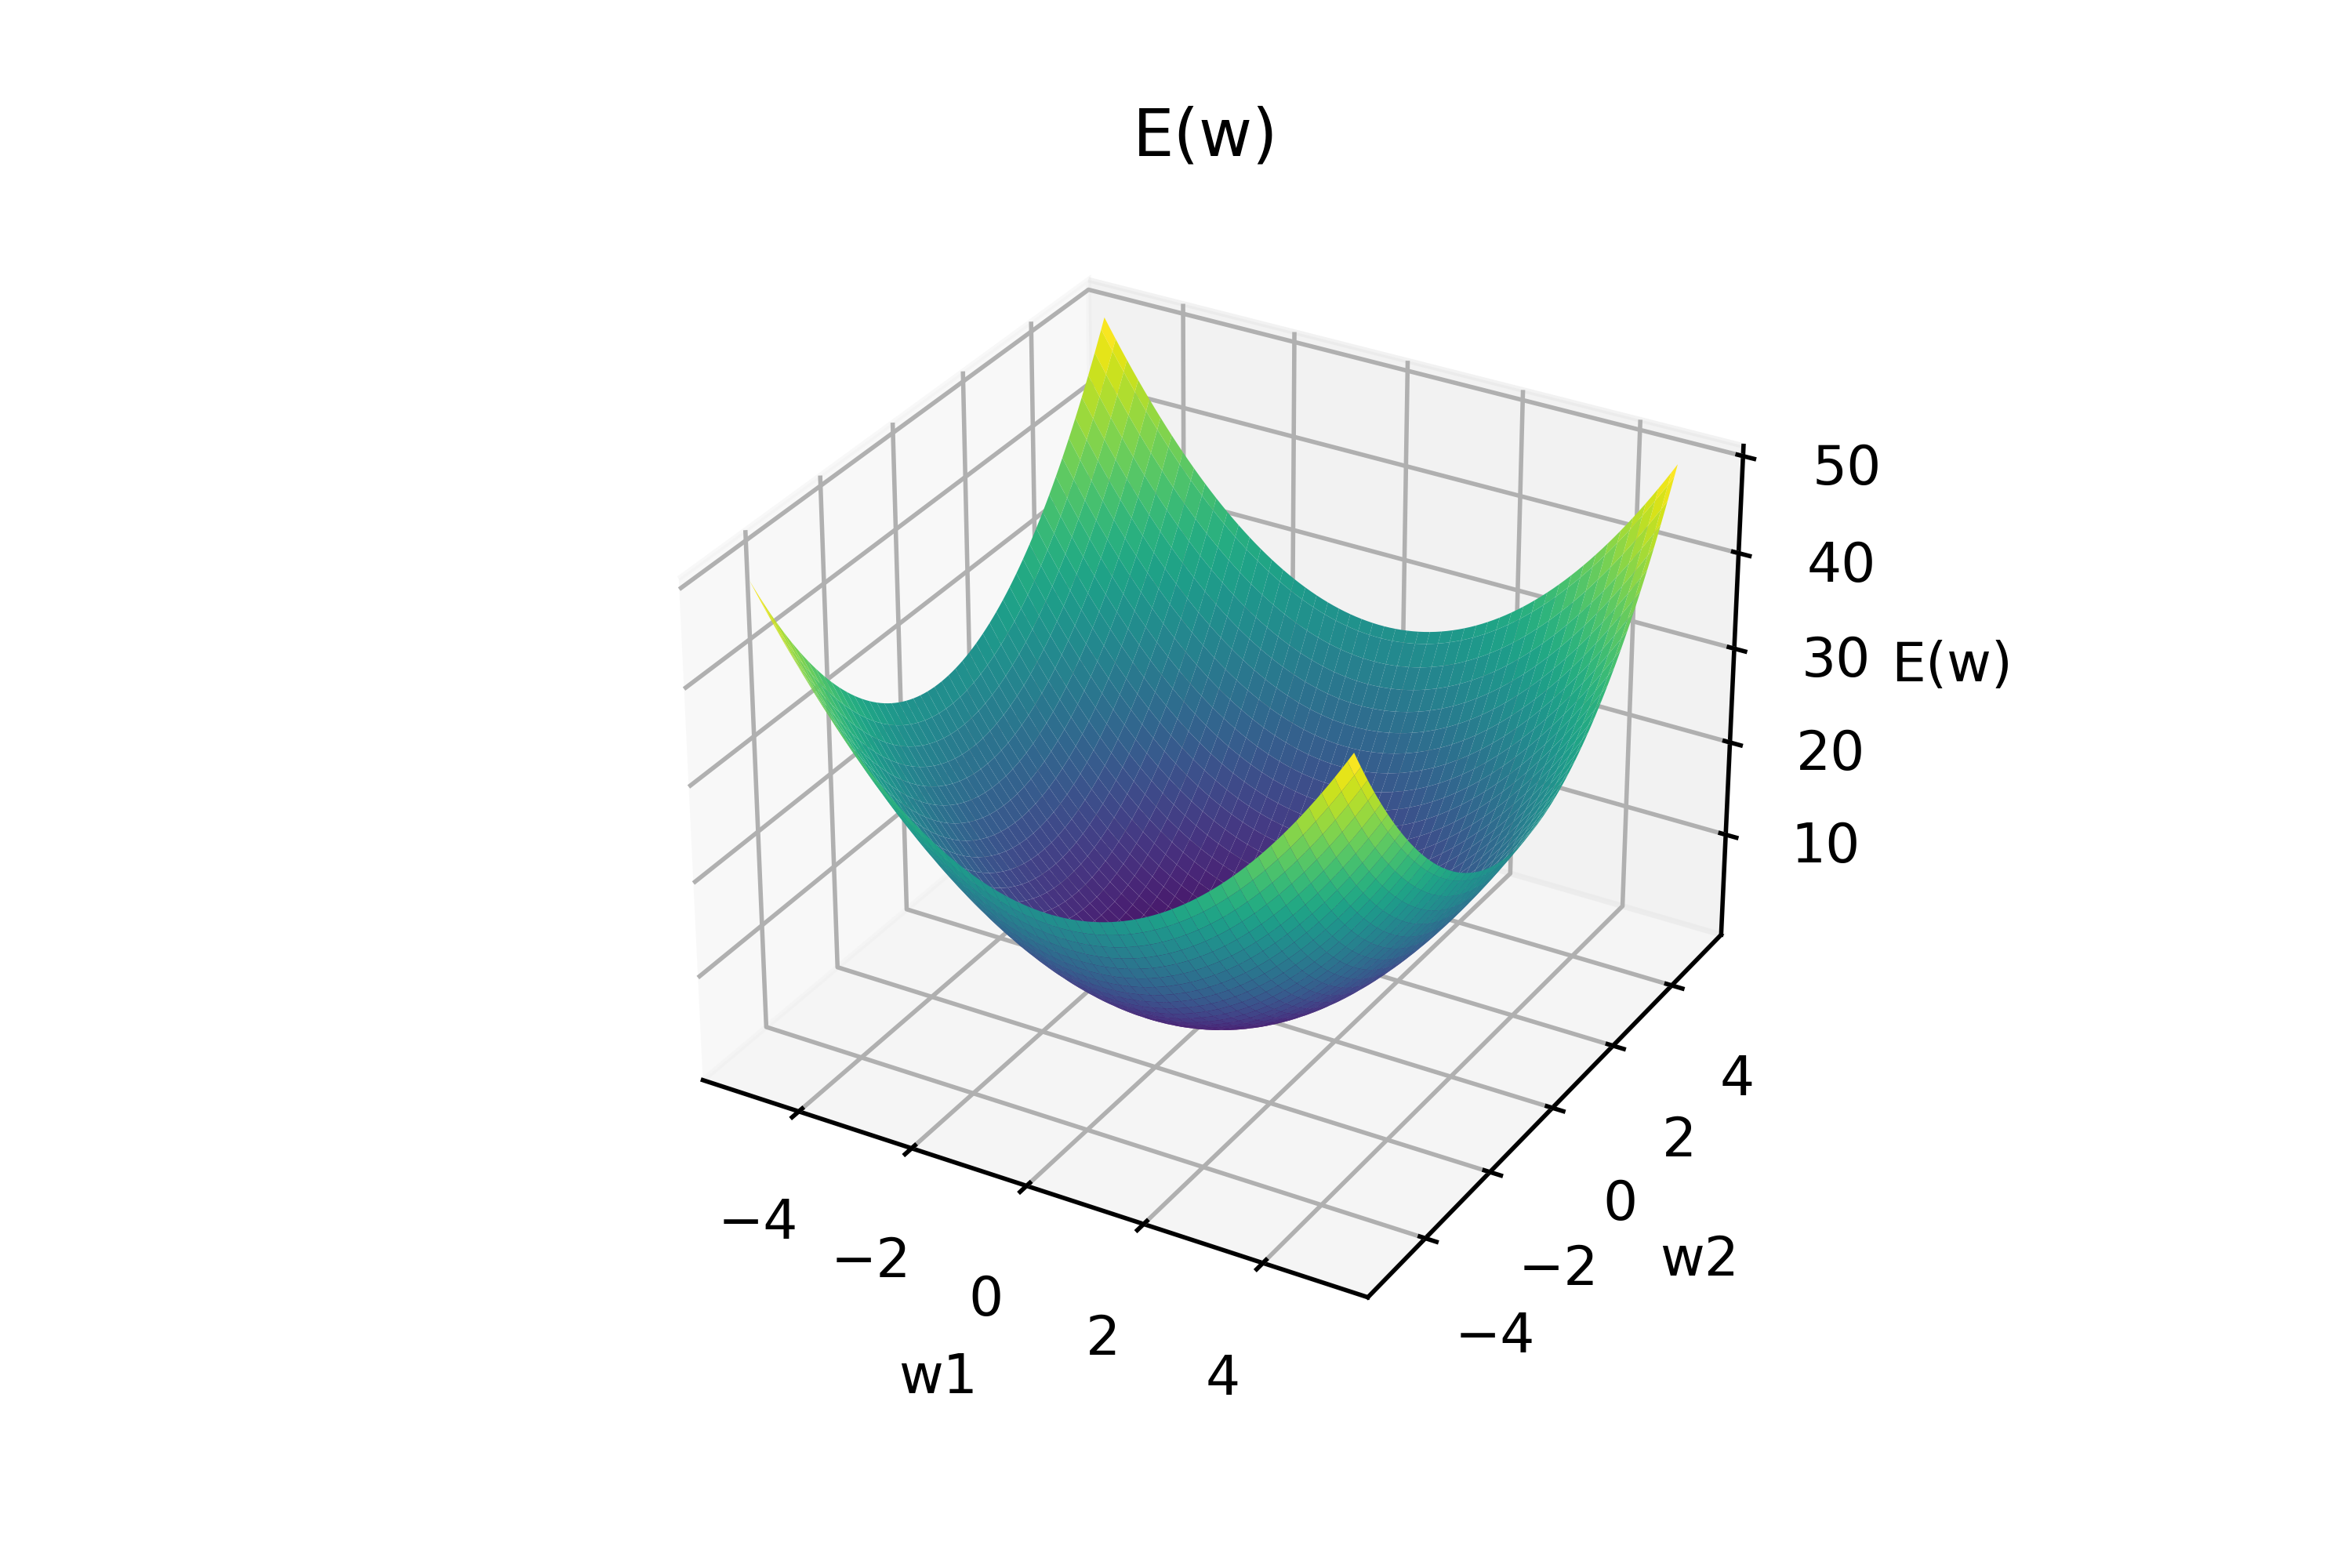
\includegraphics[scale=1]{imgss220.png}
	\caption{Ejemplo de Función de Error E(w)}
	\label{fig:figura700_10}
\end{figure}

Dado que una función de error tendrá una alta dependencia no lineal sobre los pesos y los términos bias de la red, sobre la función se pueden llegar a presentar diversos puntos en los que el gradiente se desvanezca, o numéricamente 
tenga una magnitud muy pequeña. Un punto mínimo que corresponda al valor más pequeño que pueda tomar la función de error dado un conjunto específico de pesos y bias, se conoce como \textit{mínimo global}. Existen otros puntos 
donde la función toma valores muy pequeños, sin embargo no llegan a ser los valores más pequeños posibles; a ellos se les conoce como \textit{mínimos locales}, es decir, son valores mínimos en una región especifica
de la superficie de la función de error, pero no son los valores más pequeños si se considera toda la superficie dada por la función \textit{E}(w) \cite{bishop}.  

Para lograr que una red neuronal tenga un rendimiento satisfactorio, no siempre será necesario que se encuentre el valor mínimo global para la función de error, debido a que \textit{E}(w) no se conoce. De forma general, se vuelve complicado conocer con exactitud 
si el mínimo hallado en el entrenamiento del modelo es el mínimo global, por lo tanto siempre se vuelve importante buscar o considerar diversos puntos que generen valores pequeños para \textit{E}\textbf{(w)}, y realizar 
la comparativa entre ellos para elegir la mejor optimización para los pesos y los términos bias \cite{bishop}.

Otro inconveniente en la optimización de los pesos y bias de una red neuronal, surge en el hecho de que generalmente resulta imposible hallar unsa solución análitica para la ecuación (\ref{eq:ecuacion733}), por lo tanto 
el camino preferido en estos casos es recurrir a soluciones generadas por métodos numéricos. Los problemas de optimización para funciones no lineales es un problema de estudio que puede llevar a múltiples propuestas de solución
generadas con el paso del tiempo para casos generales o problemas muy específicos; muchas técnicas de amplio uso sugieren tomar un valor inicial para los pesos y dar pasos a través del espacio generado buscando diferentes 
combinaciones, tales como las diferentes variaciones para los algoritmos de Newton-Raphson de la forma (\ref{eq:ecuacion734}), en la cual el superíndice $\tau$ se utiliza para hacer referencia a valores futuros y actuales en los parámetros que se busca optimizar \cite{bishop}.

\begin{equation}
	\textbf{w}^{\tau + 1}=\textbf{w}^{\tau} + \Delta \textbf{w}^{\tau}  
	\label{eq:ecuacion734}
\end{equation}

Es decir, generar valores futuros mediente la adición de cambios a un valor actual de dichos pesos, y que dicho cambio sea dependiente también del valor actual para los pesos. En algoritmos de optimización de este tipo
resulta buena elección tomar la información dada por el gradiente de la función de error para generar los cambios que serán necesarios aplicar para generar valores nuevos de los pesos partiendo de valores anteriores.

En el entrenamiento de redes neuronales, el uso de la información proporcionada por el gradiente de la función de error es un recurso que puede llevar a mejoras significativas en la velocidad con la cual se pueden localizar 
los valores mínimos de la función. El uso del gradiente para optimización de una red neuronal consiste en generar la actualización de los pesos, la cual debe estar condicionada por el inverso aditivo del gradiente de la función 
de error, es decir, avanzar en una dirección que nos acerque a puntos mínimos \cite{bishop}. La ecuación (\ref{eq:ecuacion735}) retrata lo descrito anteriormente.

\begin{equation}
	\textbf{w}^{\tau + 1}=\textbf{w}^{\tau} - \eta \nabla E(\textbf{w}^{\tau})
	\label{eq:ecuacion735}
\end{equation}

Lo que nos indica la ecuación (\ref{eq:ecuacion735}) es que un valor futuro o actualizado de los pesos se puede obtener a partir del valor actual de los mismos, y a dicho factor se le debe restar una \textit{porción} del 
vector gradiente generado en la función de error para los valores actuales. El factor $\eta$ se conoce como \textit{learning rate} o {tasa de aprendizaje}, el cual nos ayuda a controlar la rapidez de optimización 
al dar saltos más grandes o más pequeños sobre la superficie de la función de error en la búsqueda de valores mínimos; esta ecuación de optimización debe ejecutarse de manera iterativa para cada dato de entrenamiento introducido 
a la red \cite{bishop}. 

La actualización de los pesos de una red neuronal de la forma (\ref{eq:ecuacion735}) implica al mismo tiempo en cada iteración del algoritmo una propagación \textit{proporcional} del error a la salida del modelo, hacia las 
capas anteriores de la red (\textit{error backpropagation}). Es decir, la ecuación (\ref{eq:ecuacion735}) únicamente nos dice la regla general a seguir al actualizar un valor, sin embargo, el error dado a la salida debe distribuirse por toda la red. Lo 
anterior significa que al tener un conjunto de pesos sinápticos en el modelo, no todos ellos son responsables en la misma proporción de la magnitud del error generado, cada uno de ellos aporta mayor o menor \textit{responsabilidad} 
sobre el error total.

La mayoría de los métodos de entrenamiento usan técnicas iterativas de minimización de una función de error, realizando ajustes a los pesos conforme el algoritmo se ejecuta paso a paso. En estos algoritmos es posible identificar 
2 diferentes etapas; la primera etapa, en la cual las derivadas de la función de error son evaluadas con respecto a los valores de los pesos. En esta parte la contribución dada por las técnicas de propagación hacia atrás 
reside en generar métodos eficientes a nivel computacional para poder evaluar las derivadas. En la segunda etapa, las derivadas del error son utilizadas para el cálculo de los ajustes o actualización sobre los valores de 
los pesos de la red \cite{bishop}.

El propósito para esta última parte del capítulo es obtener las ecuaciones generales para un algortimo de propagación hacia atrás del error en una red neuronal de topología arbitraria de propagación hacia adelante, así como 
tambien funciones no lineales de activación arbitrarias y una amplia posibilidad de tipos de función de error. Primeramente se define una función de error \textit{E}\textbf{(w)} como la suma de errores individuales para cada 
vector de caracteristicas de entrenamiento (\ref{eq:ecuacion736}).

\begin{equation}
	E(\textbf{w})=\sum_{n=1}^{N} {E_{n} (\textbf{w})}
	\label{eq:ecuacion736}
\end{equation}

Donde un vector de entrenamiento tiene la forma (\ref{eq:ecuacion101736}):

\begin{equation}
	\textbf{x}=(x_{1},x_{2}, \cdot \cdot \cdot , x_{D} )
	\label{eq:ecuacion101736}
\end{equation}

La función de error para un vector de datos de entrada toma la forma (\ref{eq:ecuacion737}).

\begin{equation}
	E_n=\frac{1}{2} \sum_{}^{} {(y_{nk} - t_{nk})}^2
	\label{eq:ecuacion737}
\end{equation}

donde 

\begin{equation}
	y_{nk}=y_{k} (\textbf{x}_{n},\textbf{w})
	\label{eq:ecuacion738}
\end{equation}

es decir, el valor de la salida de la red para un valor específico de datos de entrada y pesos sinápticos. El gradiente de esta función de error viene dado por la ecuación (\ref{eq:ecuacion739}).

\begin{equation}
	\frac{\partial{E_n}}{\partial{w_{ji}}}=\frac{1}{2} \frac{\partial{{(y_{nk} - t_{nk})}^2}}{\partial{w_{ji}}}
	\label{eq:ecuacion567739}
\end{equation}

\begin{equation}
	%\frac{\partial{E_n}}{\partial{w_{ji}}}=\frac{\partial{{(\sum_{i}^{} {w_{ki}x_{i}} - t_{nk})}^2}}{\partial{w_{ji}}}
	\frac{\partial{E_n}}{\partial{w_{ji}}}=({y_{nk} - t_{nk}}) \frac{\partial{({y_{nk} - t_{nk}})}}{\partial{w_{ji}}}
	\label{eq:ecuacion567738}
\end{equation}

El término del target es 0 al derivarse al no depender de los pesos.

\begin{equation}
	\frac{\partial{E_n}}{\partial{w_{ji}}}=({y_{nk} - t_{nk}}) \frac{\partial{y_{nk}}}{\partial{w_{ji}}}
	\label{eq:ecuacion567737}
\end{equation}

Sustituyendo al valor estimado por el modelo como una combinación lineal de datos de entrada:

\begin{equation}
	\frac{\partial{E_n}}{\partial{w_{ji}}}=({y_{nk} - t_{nk}}) \frac{\partial{\sum_{i}^{} {w_{ji}x_{n}}}}{\partial{w_{ji}}}
	\label{eq:ecuacion567736}
\end{equation}

Al derivar, el valor $x_n$ es constante, por lo tanto queda la derivada del peso con respecto a sí mismo, cuyo resultado es 1, quedando la forma final:

\begin{equation}
	\frac{\partial{E_n}}{\partial{w_{ji}}}=(y_{nk} - t_{nk}) x_{n}
	\label{eq:ecuacion739}
\end{equation}

La ecuación (\ref{eq:ecuacion739}) se puede interpretar como un cálculo \textit{puntual} que involucra el producto de una señal que representa un error puntual, el cual está asociado al extremo de salida de un enlace sináptico 
en la red y un dato \textit{x} asociado al extremo de entrada de dicho enlace. A partir de este simple resultado se pueden generar ecuaciones que trabajen para redes multicapa. 

Hay que recordar que un nodo o neurona individual realiza el cálculo de una combinación lineal dada por sus pesos de enlace específicos de la forma (\ref{eq:ecuacion740}).

\begin{equation}
	a_j=\sum_{i}^{} {w_{ji} z_{i}}
	\label{eq:ecuacion740}
\end{equation}

y a la sumatoria en (\ref{eq:ecuacion740}) se le realiza una transformación no lineal de la forma (\ref{eq:ecuacion741}).

\begin{equation}
	z_j=h(a_j)
	\label{eq:ecuacion741}
\end{equation}

Tal como se muestra en la \autoref{fig:figura70010As}:

\begin{figure}[h]
	\centering
	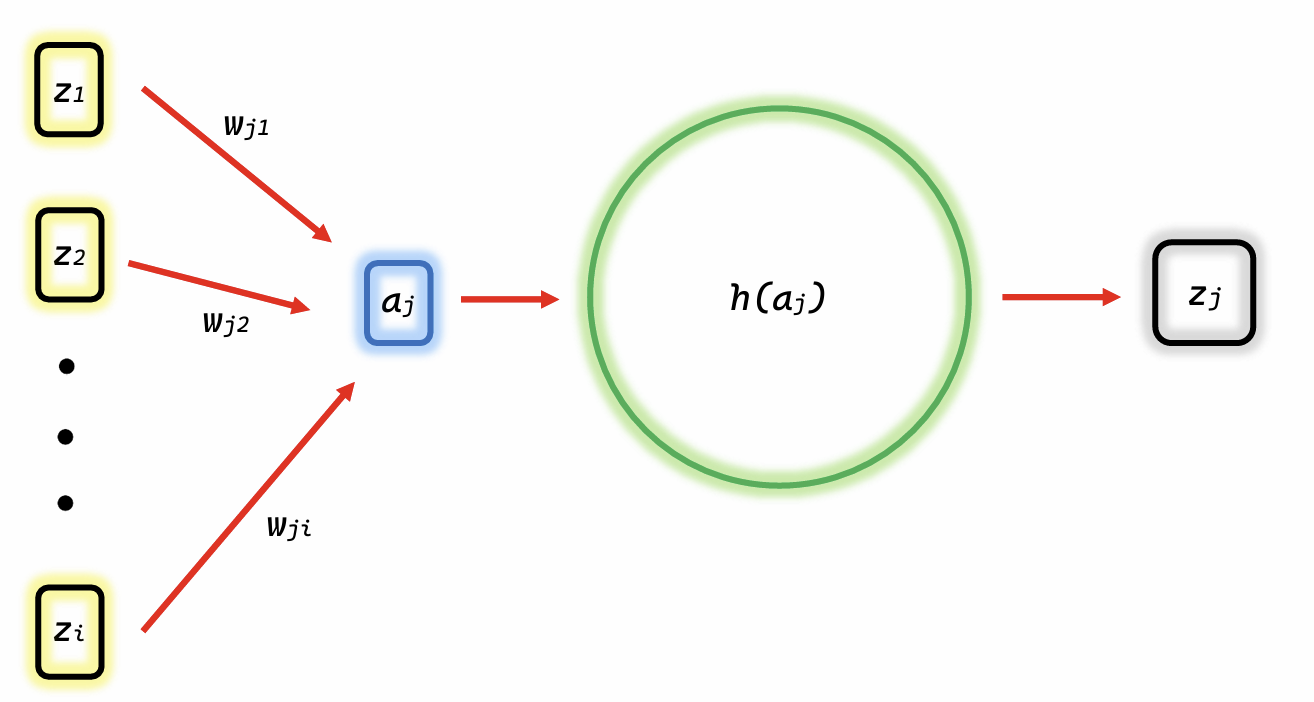
\includegraphics[scale=0.7]{imgss221.png}
	\caption{Representación de la operación de un nodo individual}
	\label{fig:figura70010As}
\end{figure}

La correcta aplicación de las ecuaciones (\ref{eq:ecuacion740}) y (\ref{eq:ecuacion741}) para cada vector de características significa el haber calculado todas las combinaciones lineales y señales de salida de cada uno de 
los nodos de la capa de salida y todas las capas ocultas presentes. Ahora consideremos la derivada de \textit{$E_n$} con respecto a un peso cualquiera; el error \textit{$E_n$} depende siempre del peso de enlace previo a través 
de la activación \textit{$a_j$} que es entrada al j-ésimo nodo. Dado lo anterior sobre la dependencia de \textit{$E_n$} con el peso de enlace previo y entrada de activación previa, al aplicar la derivada se puede hacer uso de 
la regla cadena para generar la ecuación (\ref{eq:ecuacion742}).

\begin{equation}
	\frac{\partial{E_n (w_{ji})}}{\partial{w_{ji}}}=\frac{\partial{E_n}}{\partial{a_{j}}} \frac{\partial{a_j}}{\partial{w_{ji}}}
	\label{eq:ecuacion742}
\end{equation}

Haciendo un cambio de notación dado por (\ref{eq:ecuacion743}).

\begin{equation}
	\delta_{j}=\frac{\partial{E_n}}{\partial{a_{j}}}
	\label{eq:ecuacion743}
\end{equation}

Si la ecuación (\ref{eq:ecuacion740}) la derivamos con respecto de un peso cualquiera, nos queda el dato de entrada de la combinación lineal que no depende del valor del peso, por lo tanto resulta la expresión (\ref{eq:ecuacion744}).

\begin{equation}
	\frac{\partial{a_j}}{\partial{w_{ji}}}=z_i
	\label{eq:ecuacion744}
\end{equation}

Ahora sustituyendo las ecuaciones (\ref{eq:ecuacion743}) y (\ref{eq:ecuacion744}) en la ecuación (\ref{eq:ecuacion742}), obtenemos la expresión simplificada (\ref{eq:ecuacion745}).

\begin{equation}
	\frac{\partial{E_n}}{\partial{w_{ji}}}=\delta_{j} z_i
	\label{eq:ecuacion745}
\end{equation}

La ecuación (\ref{eq:ecuacion745}) nos dice que la derivada del error respecto a un peso cualquiera se obtiene al multiplicar el error parcial \textit{$\delta$} en el extremo de salida de un nodo \textit{ji}, por la activación de entrada 
en el extremo del inicio del enlace entre nodos. Por lo cual, para calcular las derivadas es necesario obtener los valores $\delta$ para cada nodo de las capas ocultas y de salida, y posteriormente aplicar la ecuación (\ref{eq:ecuacion745}).

Para los nodos de la capa de salida ya se conoce la relación dada por (\ref{eq:ecuacion746}) para el error en el k-ésimo nodo.

\begin{equation}
	\delta_{k}=y_{k} - t_k
	\label{eq:ecuacion746}
\end{equation}

Para los nodos de las capas ocultas, el cálculo de los valores $\delta$ para cada capa implica volver a aplicar la regla de la cadena (\ref{eq:ecuacion747})

\begin{equation}
	\delta_{j}=\frac{\partial{E_n}}{\partial{a_{j}}}=\sum_{k}^{} {\frac{\partial{E_n}}{\partial{a_{k}}} \frac{\partial{a_k}}{\partial{a_{j}}}}
	\label{eq:ecuacion747}
\end{equation}

donde la sumatoria se aplica sobre todos los nodos de la k-ésima capa a los cuales un nodo de la j-ésima capa previa envía una conexión sináptica. Cuando se habla de k-ésima capa se hace referencia a que esta capa puede ser 
capa de salida o capa oculta. Si en la ecuación (\ref{eq:ecuacion747}) se usa (\ref{eq:ecuacion743}) para hacer la substitución de la derivada parcial del error por el valor $\delta$ y posteriormente 
se usan las ecuaciones (\ref{eq:ecuacion740}) y (\ref{eq:ecuacion741}) para sustituir por la derivada parcial de la k-ésima entrada de activación, se puede llegar a una ecuación general de propagación hacia atrás del error.

\begin{equation}
	\delta_{k}=\frac{\partial{E_n}}{\partial{a_{k}}}
	\label{eq:ecuacion748}
\end{equation}

\begin{equation}
	\frac{\partial{a_k}}{\partial{a_{j}}}=\frac{\partial{\sum_{k}^{} {w_{kj} z_j}}}{\partial{a_{j}}}
	\label{eq:ecuacion749}
\end{equation}

Desarrollando (\ref{eq:ecuacion749})

\begin{equation}
	\frac{\partial{a_k}}{\partial{a_{j}}}=\frac{\partial{\sum_{k}^{} {w_{kj} h(a_j)}}}{\partial{a_{j}}}
	\label{eq:ecuacion750}
\end{equation}

La derivada puede introducirse en la sumatoria

\begin{equation}
	\frac{\partial{a_k}}{\partial{a_{j}}}=\sum_{k}^{} {\frac{\partial{w_{kj} h(a_j)}}{\partial{a_{j}}}}
	\label{eq:ecuacion751}
\end{equation}

El peso \textit{w} al no depender de \textit{$a_j$} puede salir de la derivada

\begin{equation}
	\frac{\partial{a_k}}{\partial{a_{j}}}=\sum_{k}^{} {w_{kj} \frac{\partial{h(a_j)}}{\partial{a_{j}}}}
	\label{eq:ecuacion752}
\end{equation}

La derivada, al no tener dependencia sobre el subíndice \textit{k}, puede salir de la sumatoria 

\begin{equation}
	\frac{\partial{a_k}}{\partial{a_{j}}}=\frac{\partial{h(a_j)}}{\partial{a_{j}}} \sum_{k}^{} {w_{kj}} 
	\label{eq:ecuacion753}
\end{equation}

Finalmente, sustituyendo los resultados (\ref{eq:ecuacion753}) y (\ref{eq:ecuacion748}) en la ecuación (\ref{eq:ecuacion747}) se llega al resultado (\ref{eq:ecuacion754})

\begin{equation}
	\delta_{j}=\frac{\partial{h(a_j)}}{\partial{a_{j}}} \sum_{k}^{} {w_{kj} \delta_{k}} 
	\label{eq:ecuacion754}
\end{equation}

%La ecuación (\ref{eq:ecuacion754}) representa un método general para la propagación hacia atrás del error en una red neuronal y nos dice que el error parcial en un nodo de una capa oculta se puede obtener al propagar hacia 
%atrás los errores de capas posteriores. Por lo tanto los pasos a seguir para el ajuste de una red neuronal son los siguientes:

La ecuación (\ref{eq:ecuacion754}) representa una expresión general para el cálculo de los errores proporcionales para las capas ocultas. Este resultado nos permite el uso de la ecuación (\ref{eq:ecuacion745}) para el cálculo 
de las derivadas del error con respecto a los pesos correspondientes, lo cual es requerido para la ecuación de Newton-Raphson para actualización de los pesos. 

Por último, se debe señalar que en la ecuación (\ref{eq:ecuacion754}), al ser una forma general, ya en la práctica se debe tener en cuenta que diferentes capas de la red neuronal pueden tener diferentes funciones de activación, 
por lo cual al usar dicha ecuación debe usarse la correspondiente función de activación que exista en la capa de la red donde se estén realizando los ajustes.

De forma general, el procedimiento para el ajuste de una red neuronal es el siguiente:

\begin{lstlisting}[language=Python,numbers=none]
	DEFINIR NUMERO DE ENTRADAS 
	input_nodes:A

	DEFINIR NUMERO DE SALIDAS
	output_nodes:B

	DEFINIR CAPAS OCULTAS
	hidden_nodes:C

	INICIALIZAR PESOS DE LA RED CON DISTRIBUCION NORMAL COMO REFERENCIA
	wih:numpy.random.normal(0.0,pow(self.inodes,-0.5),(self.hnodes,self.inodes))
	who:numpy.random.normal(0.0,pow(self.hnodes,-0.5),(self.onodes,self.hnodes))

	DEFINIR LA TASA DE APRENDIZAJE
	lr:learningrate

	PROPAGACION HACIA ADELANTE
	hidden_inputs:numpy.dot(wih,inputs)
	hidden_outputs:self.activation_function(hidden_inputs)
	final_inputs:numpy.dot(who,hidden_outputs)
	final_outputs:self.activation_function(final_inputs)

	PROPAGACION HACIA ATRAS DEL ERROR
	output_errors:targets-final_outputs
	hidden_errors:numpy.dot(who.T,output_errors)

	ACTUALIZAR LOS PESOS
	who:who+lr*numpy.dot((output_errors*final_outputs*(1-final_outputs)),numpy.transpose(hidden_outputs))
	wih:wih+lr*numpy.dot((hidden_errors*hidden_outputs*(1-hidden_outputs)),numpy.transpose(inputs))
\end{lstlisting}

Primero es necesario definir la arquitectura de la red al establecer las capas y la cantidad de nodos en ellas. Después, se debe inicializar de forma aleatoria los pesos entre capa de entrada y capa oculta, los pesos entre 
capas ocultas y los pesos entre capa oculta y capa de salida. Al mismo tiempo es necesario establecer la tasa de aprendizaje con la cual se optimizará el modelo.

Posteriormente, se deben propagar por la red los datos de entrenamiento para obtener las estimaciones hechas con el valor actual de pesos. Finalmente, se debe hacer el cálculo de los errores en la salida de la red y los 
errores proporcionales para los pesos de capas intermedias. Con esta información se puede generar actualizaciones secuenciales sobre los pesos de la red. 

\section{Conclusiones}

En este capítulo se presentan los conceptos y desarrollo matemático para los diferentes algoritmos de inteligencia artificial que son parte del desarrollo de este trabajo. Primeramente se inicia con los conceptos fundamentales 
acerca de la regresión lineal, el cual es un método que nos permite obtener funciones matemáticas, dadas por un recta, para representar un patrón o comportamiento dado por un conjunto de datos.

Con los conceptos introducidos en las secciones dedicadas a regresión lineal, es que se identifica la necesidad de contar con métodos de ajuste para los parámetros de un modelo en específico, con el fin de obtener la mejor 
optimización. Es aquí donde se introduce el método de descenso por gradiente para minimización de una función de error dependiente de los parámetros del modelo aplicado. Este método de ajuste iterativo permite ejecutar cambios 
graduales en los parámetros del modelo utilizado hasta llegar a la mejor aproximación para el mínimo de la función de error.

Posteriormente, se desarrollan los conceptos básicos para modelos no lineales para clasificación, para después pasar con el caso específico empleado en este trabajo, que son las redes neuronales. En esta parte se explican 
las analogías entre una red biológica y una artificial, y como se van generando las ecuaciones matemáticas para nodos o neuronas individuales en la red, para posteriormente poder apilar o conjuntar nodos mediante enlaces 
por pesos para nodos de capas consecutivas en la red.

Por último, se describe un enfoque generalizado para el entrenamiento de la red neuronal artificial, describiendo mediante ecuaciones los procedimientos de propagación hacia adelante de los datos de entrenamiento y después 
la propagación hacia atrás del error a la salida del modelo, para finalmente usar la información obtenida mediante esta realimentación del error para poder hacer modificaciones en los enlaces o pesos que forman la red neuronal.

% TERMINADO YA ESTE CAPÍTULO.
